%\documentclass{beamer}
\documentclass[mathserif,10pt]{beamer}

\usepackage{beamerthemesplit}
\usepackage{graphics}
\usepackage{epsfig}
\usepackage{algorithm}
\usepackage{verbatim}
\usepackage{listings}
\usepackage{framed}
\usepackage{pstricks}
\usepackage{pst-node,pst-tree}
\usepackage{pst-rel-points}
\usepackage{flexiprogram}
\usepackage[UKenglish]{babel}
\usepackage{hyperref}
\usepackage{pst-coil}
\usepackage{color}
\usepackage{epsfig}
\usepackage{tikz}
%\usepackage{multirow}

\usefonttheme{serif}

\newcommand{\cmt}[1]{}
%\noindent

\setcounter{tocdepth}{1}
\lstset{language=[ANSI]C}
\lstset{% general command to set parameter(s)
  basicstyle=\footnotesize\tt, % print whole listing small
    identifierstyle=, % nothing happens
    commentstyle=\color{red}, % white comments
    showstringspaces=false, % no special string spaces
    lineskip=1pt,
    captionpos=b,
    frame=single,
    breaklines=true
      %\insertauthor[width={3cm},center,respectlinebreaks]
}

\setbeamercovered{transparent=50}

\lstset{classoffset=0,
  morekeywords={},keywordstyle=\color{black},
  classoffset=1,
  classoffset=0}% restore default

  \usetheme{CambridgeUS}
  \usecolortheme{dolphin}

  \title[Trace based JIT]{Trace Based Just-In-Time Type Specialization for Dynamic Languages}
  \author[]{{\textbf{Gal, Eich, Shaver, Anderson, Mandelin, Kaplan, Hoare, Zbarsky, Orendorff, Ruderman, Smith, Reitmaier, Haghighat, Bebenita, Chang, Franz}} }
  \begin{document}

  \begin{frame}
  \titlepage
  \end{frame}
  \usebeamertemplate{mytheme}

  \AtBeginSection[]
{
  \begin{frame}<beamer>
    \frametitle{Outline}
  \tableofcontents[currentsection]
    \end{frame}
}
\frame
{
  \center{
  \textbf{Name: Sandeep Dasgupta} \\
  \textbf{Advisor: Dr. Vikram Adve} \\

  Primary: Compilers  \\
  Secondary: Parallel Programming, Architecture\\
  }
}

\section{Motivation}
\subsection{Motivation}
\frame
{
  \frametitle{\subsecname}
  \begin{itemize}
  \item Generate efficient machine code for dynamic type languages like Javascript
  \end{itemize}
}

\section{Introduction}
\subsection{TraceMonkey: Proposed Compilation strategy}
\frame
{
  \frametitle{\subsecname}
  \begin{itemize}
    \item Is implemented for Javascript Interpreter SpiderMonkey
    \item{ Design Decisions}
      \begin{itemize}
        \item Dynamic compilation on loop level granularity, not method based. 
        \item No static type inferencing.
    \end{itemize}
  \end{itemize}
}
\subsection{Trace}
\frame
{
  \frametitle{\subsecname}
  \begin{itemize}
    \item Typed loop traces
    \begin{itemize}
      \item Single entry, multiple exits loop paths
      \item Type specialized
    \end{itemize}
  \end{itemize}
}
\section{Example Tracing Run}
\frame
{
  \begin{figure}[h]
  \centering
  \scalebox{0.45}{
    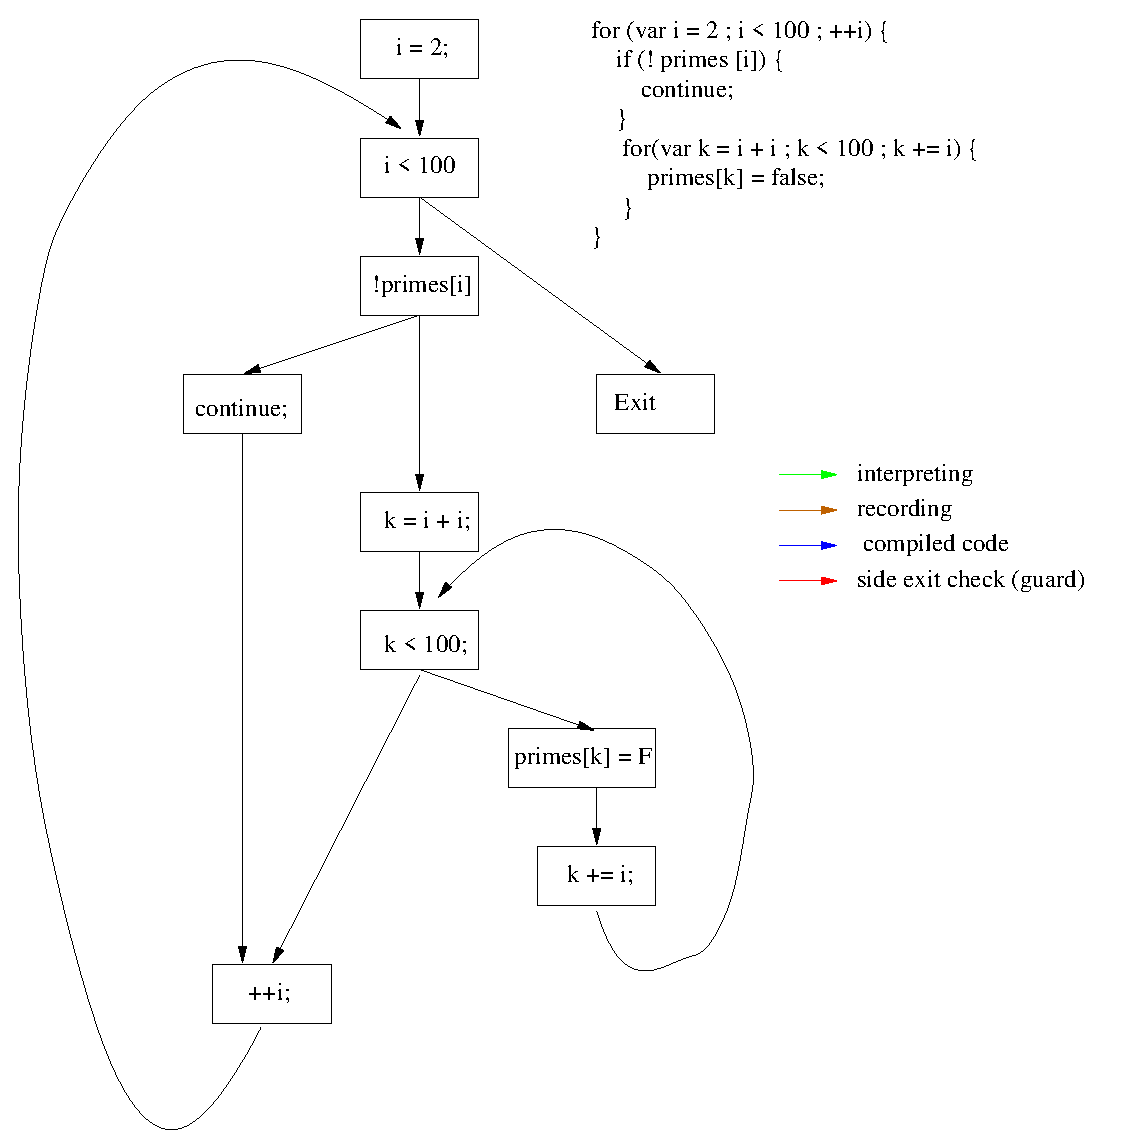
\includegraphics{Figs/1.eps}
  }
  \end{figure}
}
\frame
{
  \begin{figure}[h]
  \centering
  \scalebox{0.45}{
    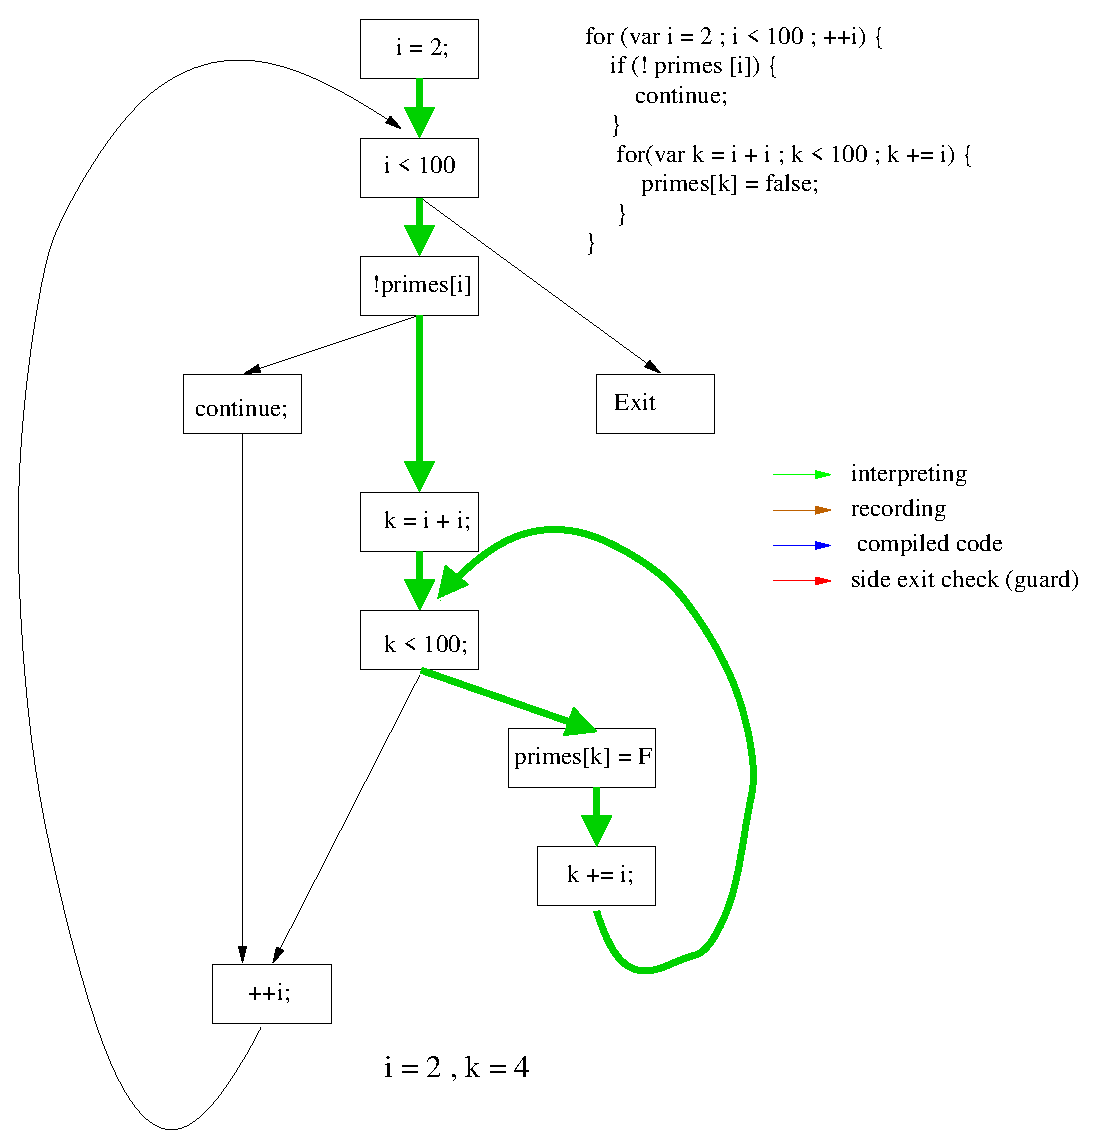
\includegraphics{Figs/1.1.eps}
  }
  \end{figure}
}
\frame
{
  \begin{figure}[h]
  \centering
  \scalebox{0.45}{
    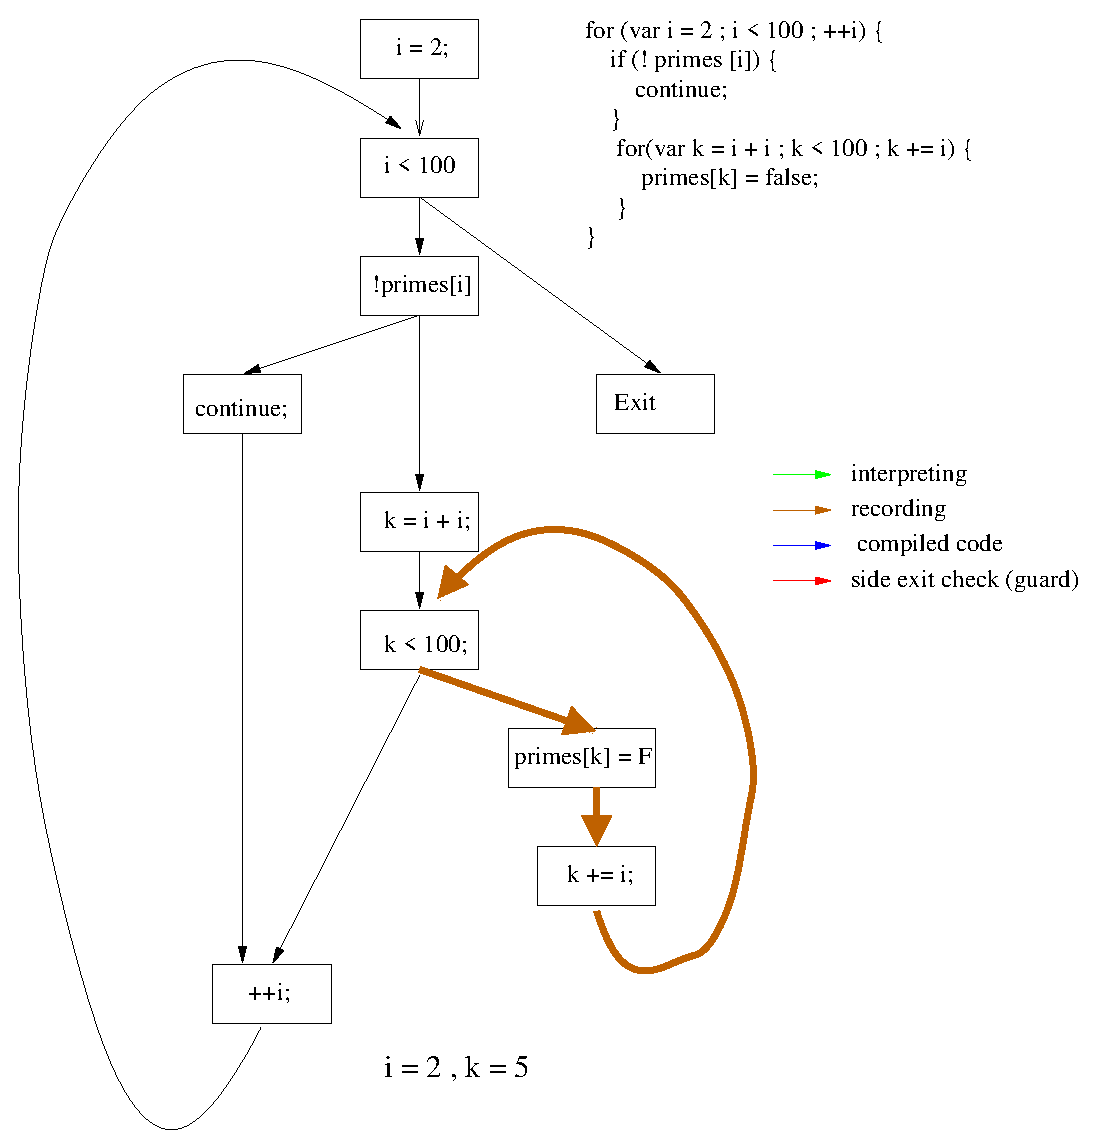
\includegraphics{Figs/1.2.eps}
  }
  \end{figure}
}
\frame
{
  \begin{figure}[h]
  \centering
  \scalebox{0.45}{
    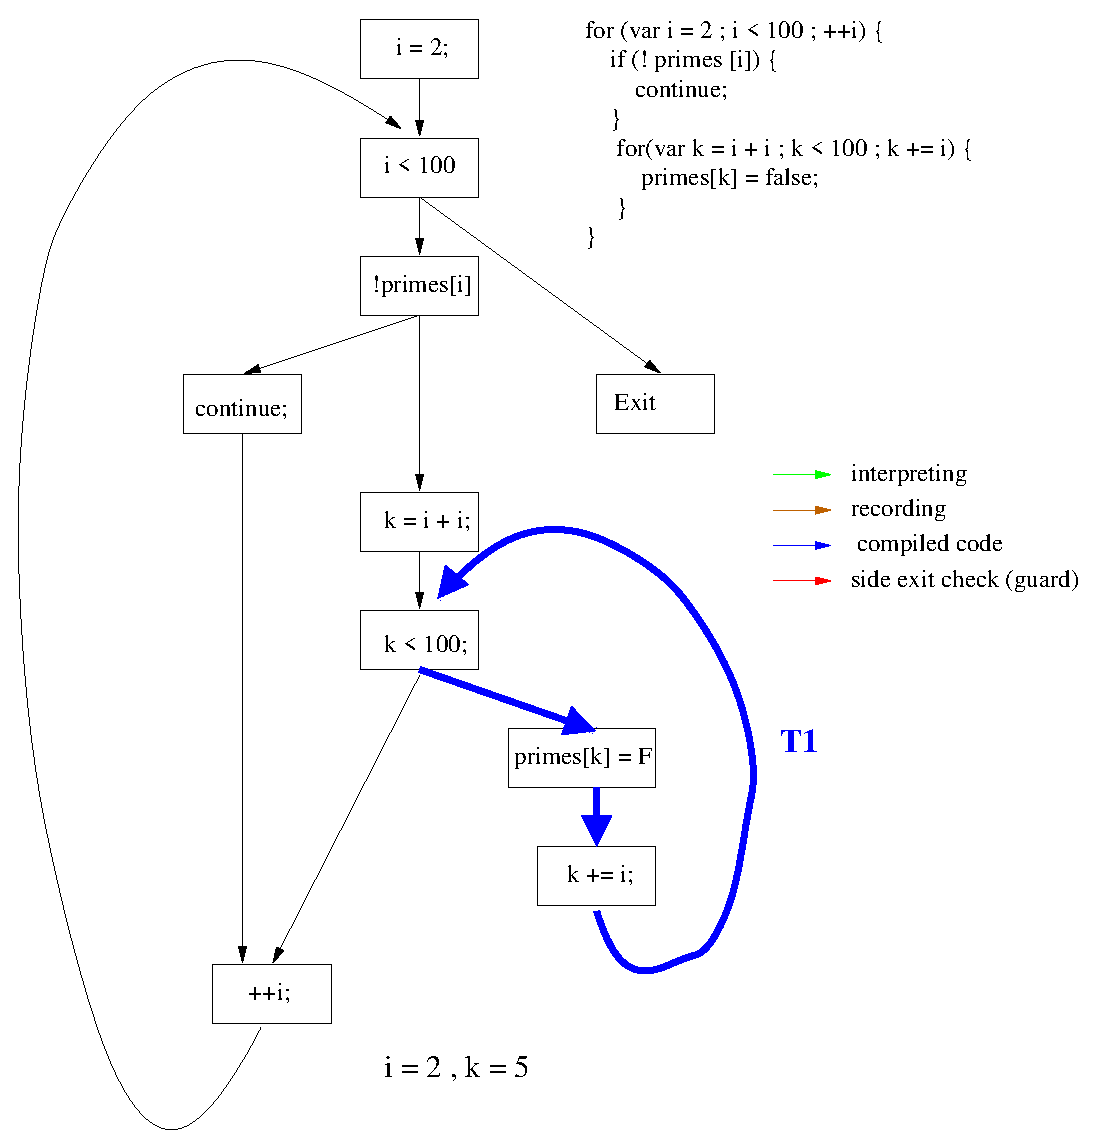
\includegraphics{Figs/1.3.eps}
  }
  \end{figure}
}
\frame
{
  \begin{figure}[h]
  \centering
  \scalebox{0.45}{
    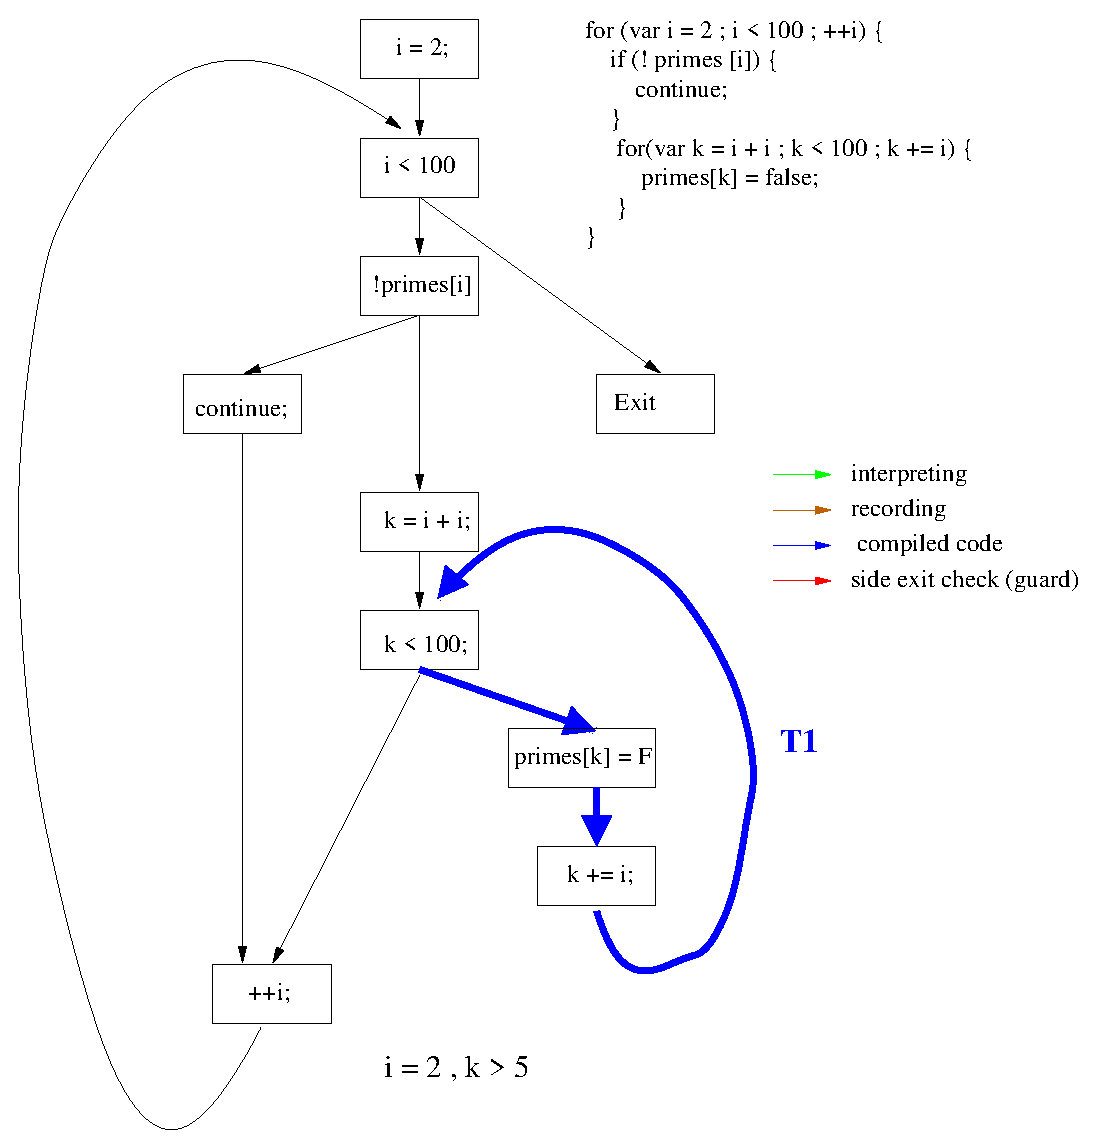
\includegraphics{Figs/1.3.1.eps}
  }
  \end{figure}
}
\frame
{
  \begin{figure}[h]
  \centering
  \scalebox{0.45}{
    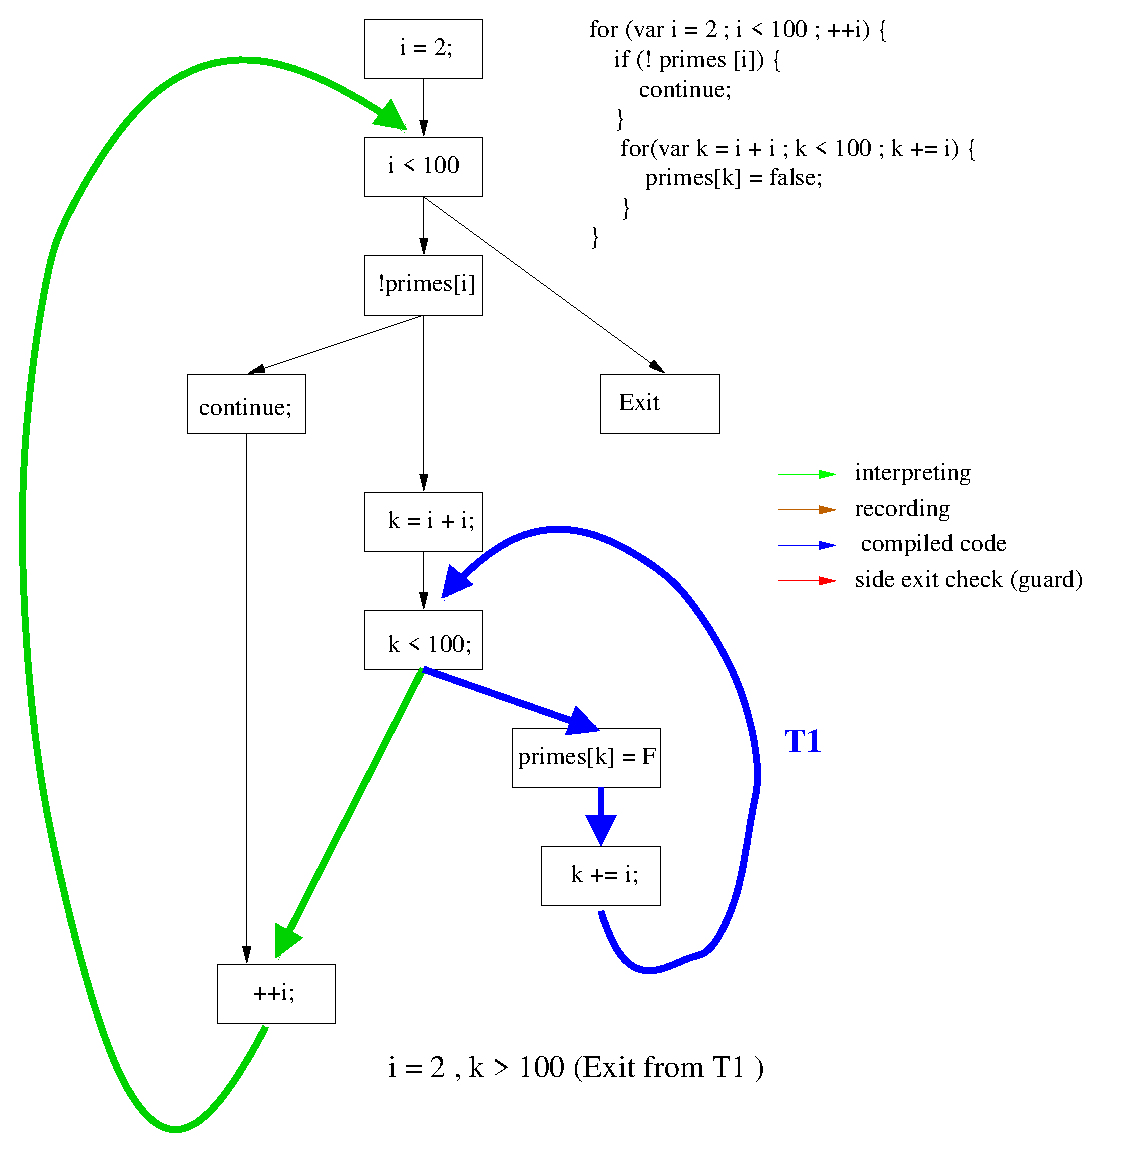
\includegraphics{Figs/1.3.2.eps}
  }
  \end{figure}
}
\frame
{
  \begin{figure}[h]
  \centering
  \scalebox{0.45}{
    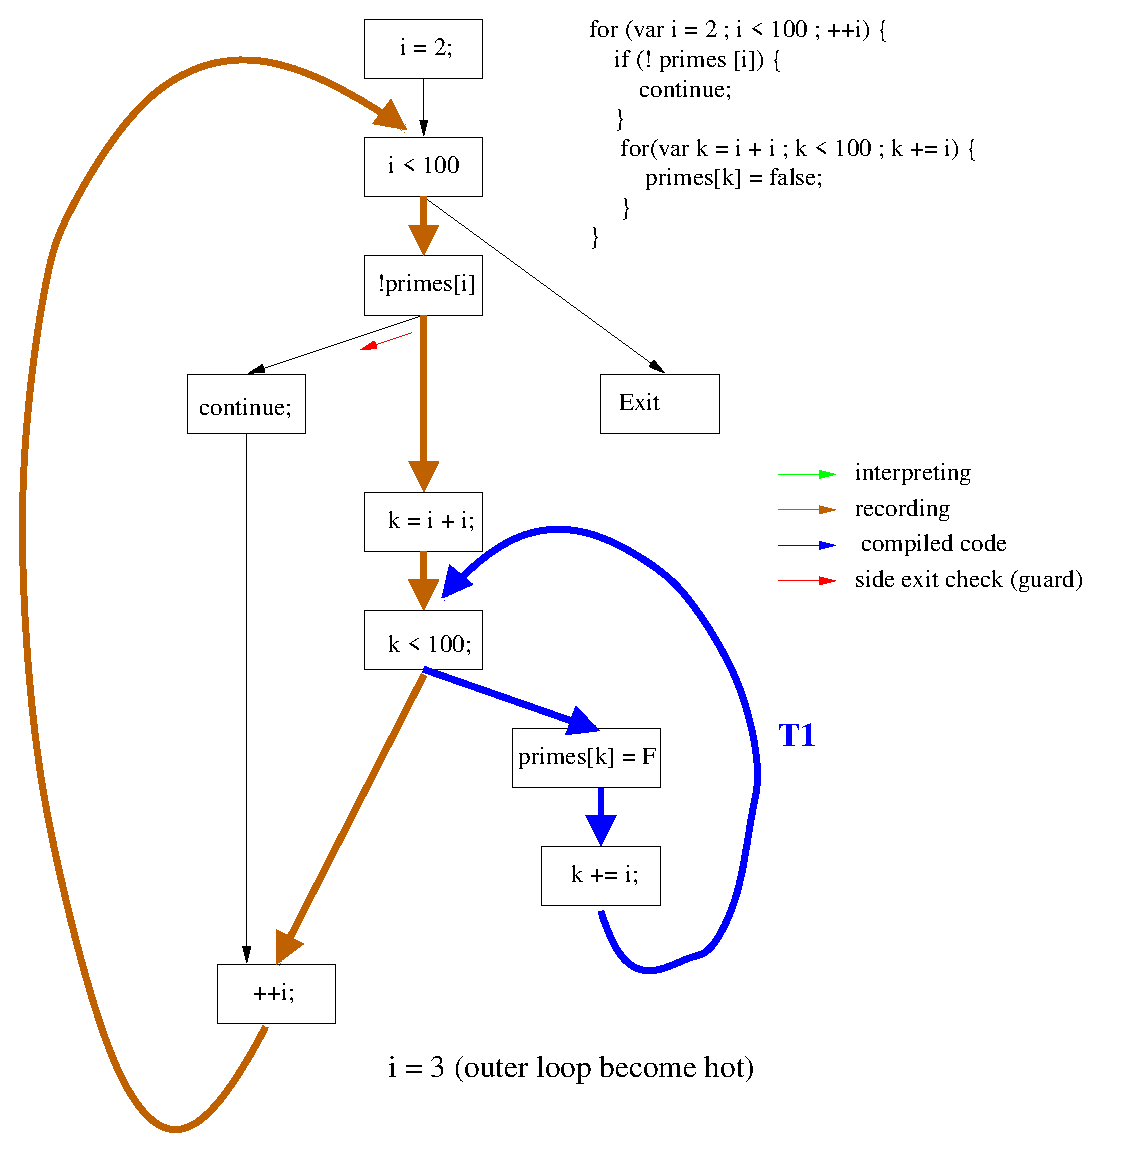
\includegraphics{Figs/1.4.eps}
  }
  \end{figure}
}
\frame
{
  \begin{figure}[h]
  \centering
  \scalebox{0.45}{
    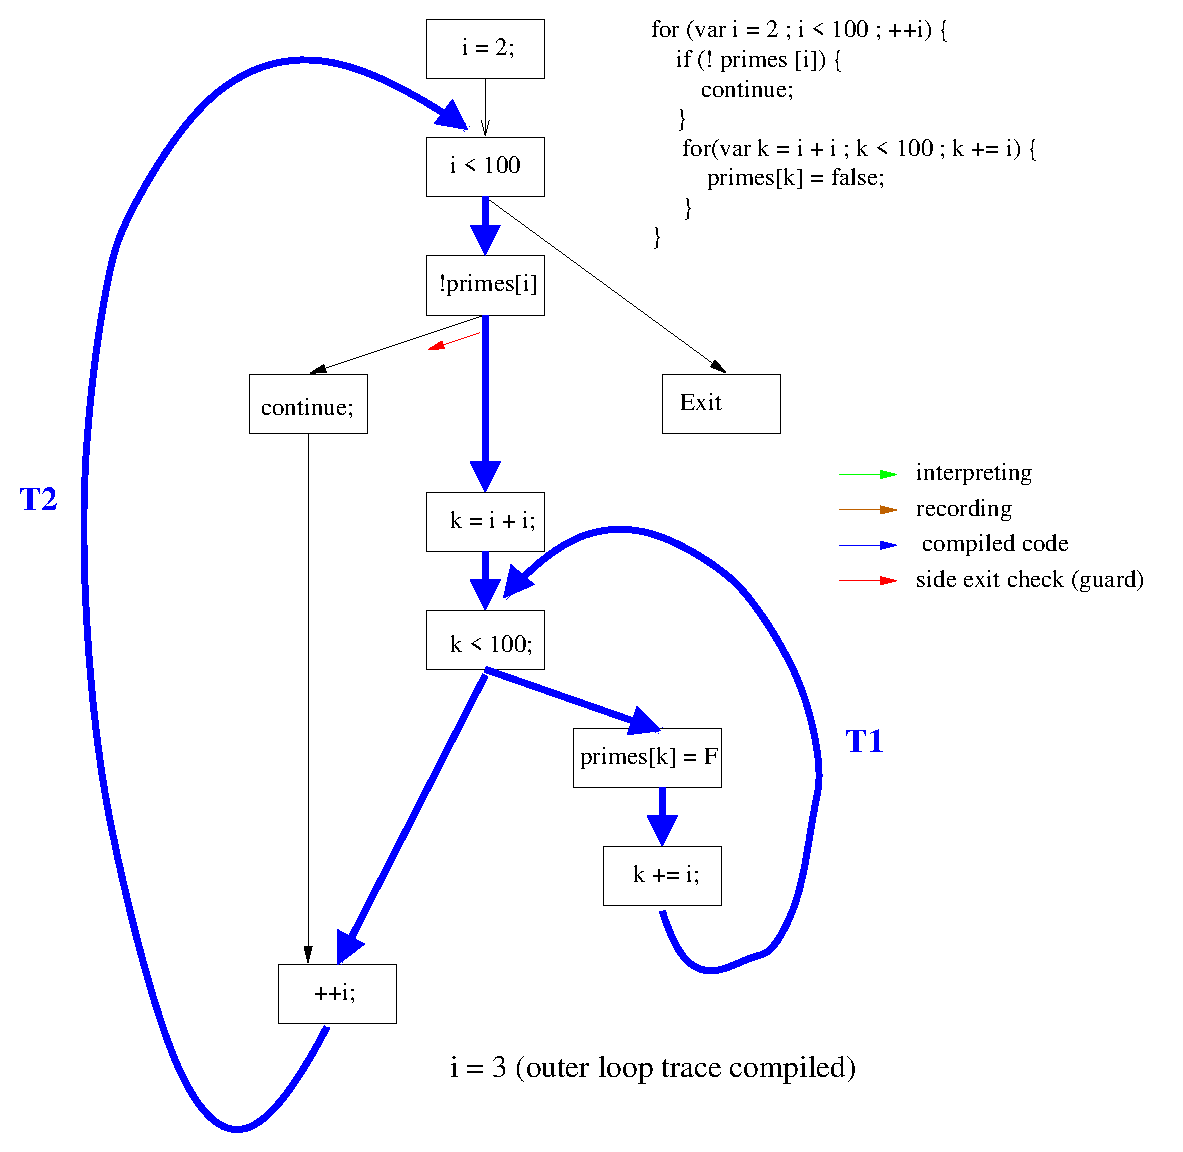
\includegraphics{Figs/1.5.eps}
  }
  \end{figure}
}
\frame
{
  \begin{figure}[h]
  \centering
  \scalebox{0.45}{
    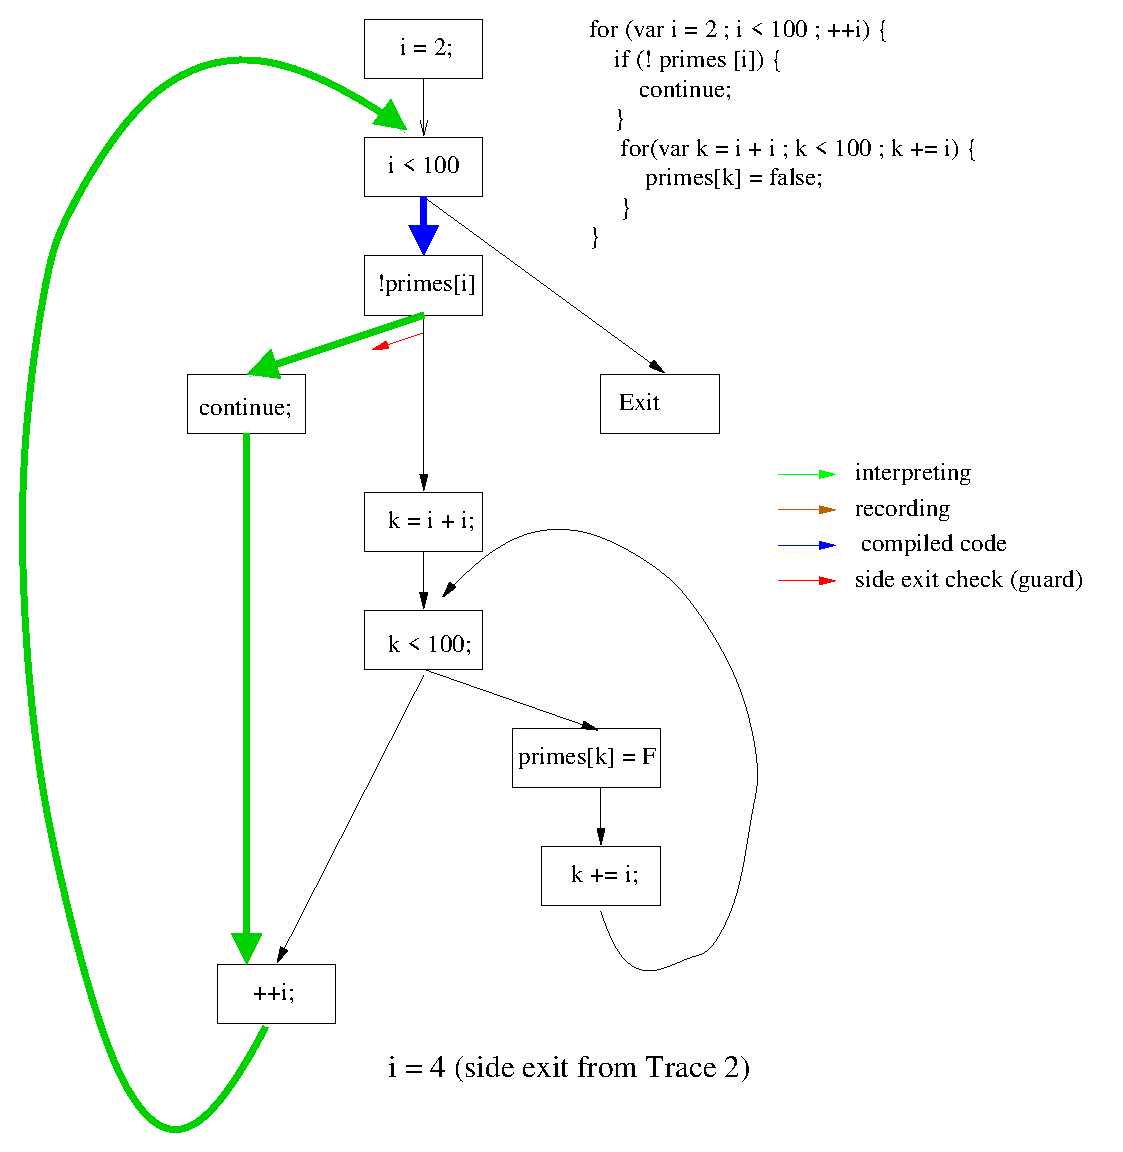
\includegraphics{Figs/1.6.eps}
  }
  \end{figure}
}
\frame
{
  \begin{figure}[h]
  \centering
  \scalebox{0.45}{
    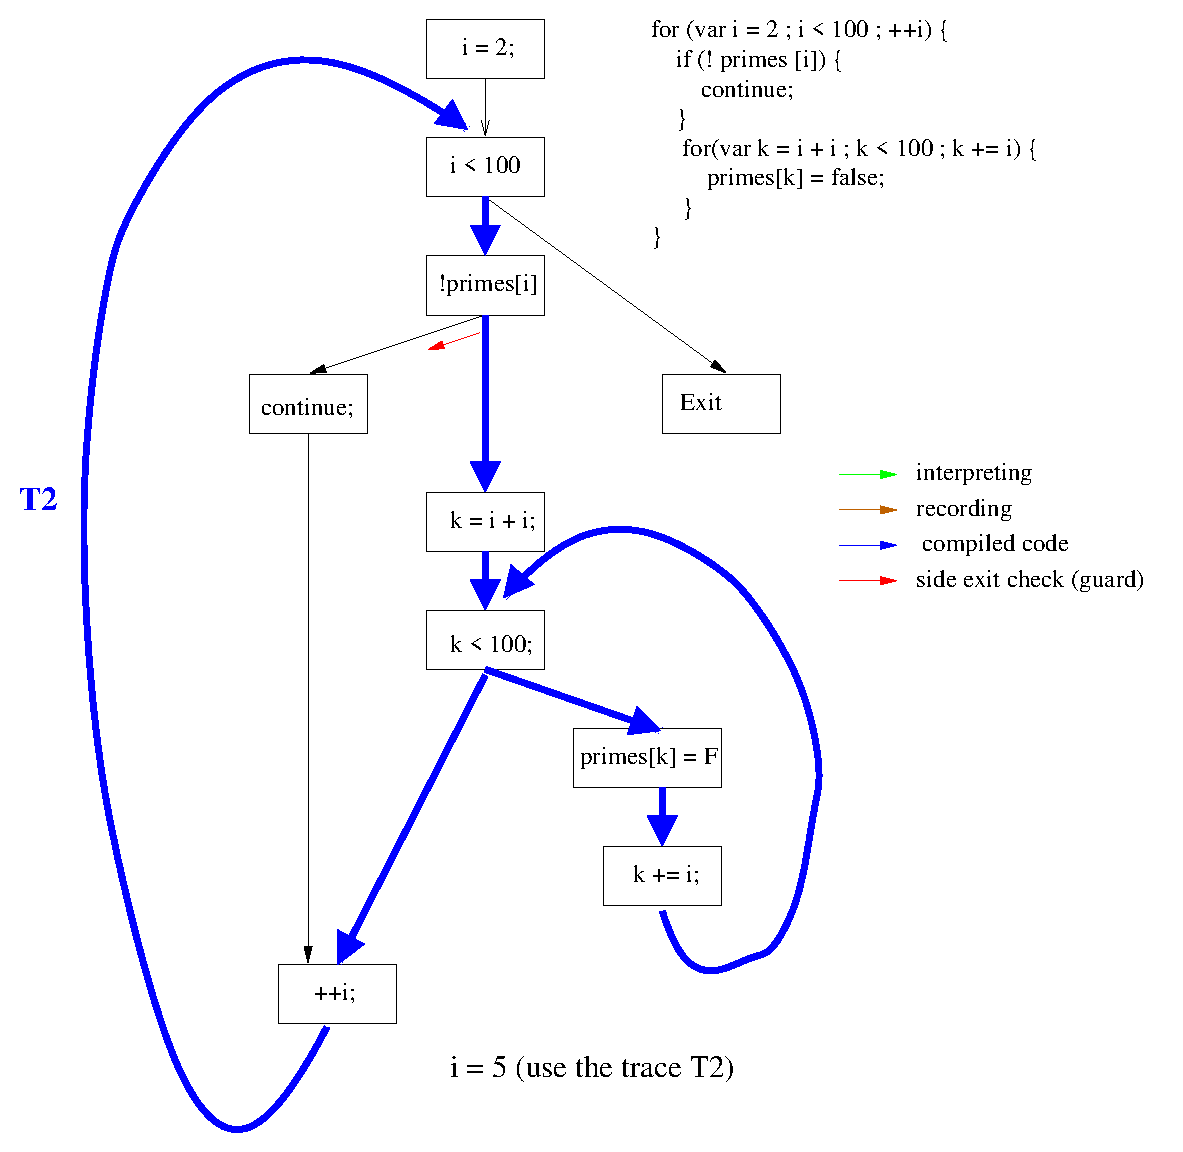
\includegraphics{Figs/1.7.eps}
  }
  \end{figure}
}
\frame
{
  \begin{figure}[h]
  \centering
  \scalebox{0.45}{
    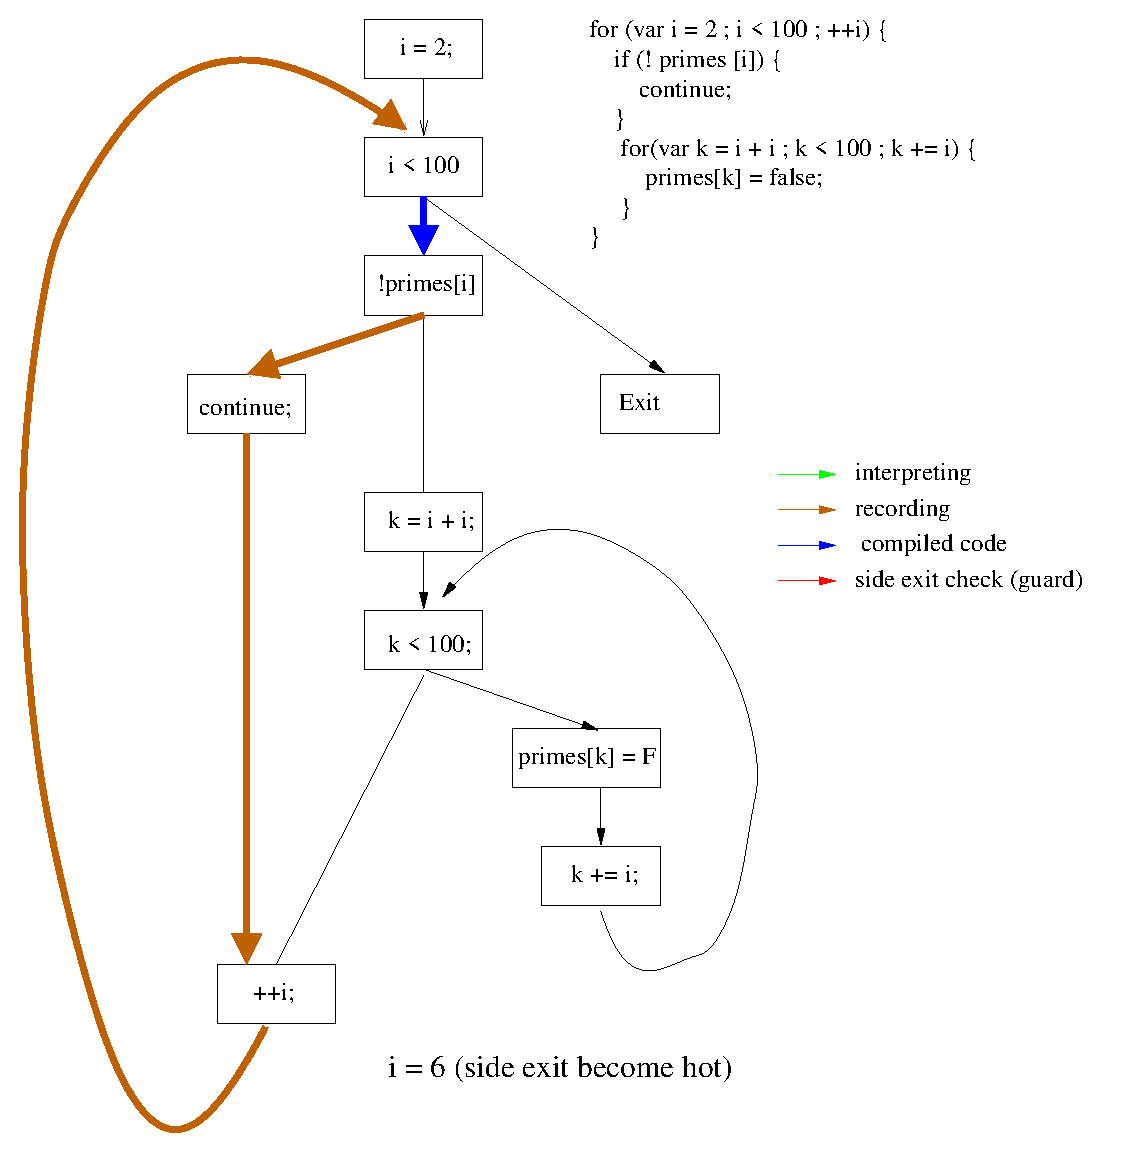
\includegraphics{Figs/1.8.eps}
  }
  \end{figure}
}
\frame
{
  \begin{figure}[h]
  \centering
  \scalebox{0.45}{
    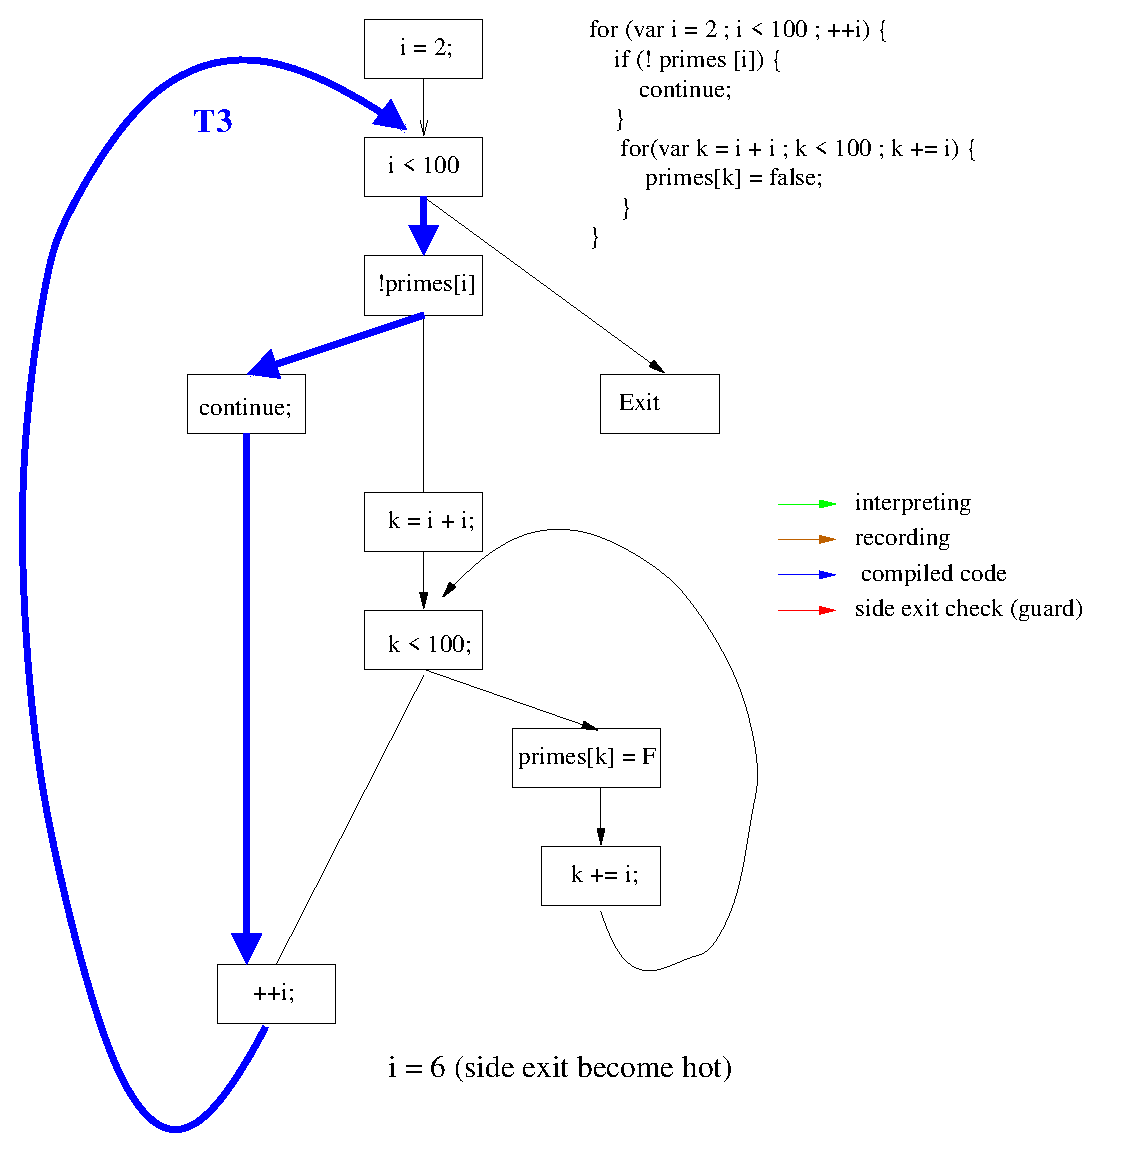
\includegraphics{Figs/1.9.eps}
  }
  \end{figure}
}

\section{Trace Tree Formation}
\subsection{Type Stable Trace}
\frame
{
  \frametitle{\subsecname}
  \begin{figure}[h]
  \centering
  \scalebox{0.45}{
    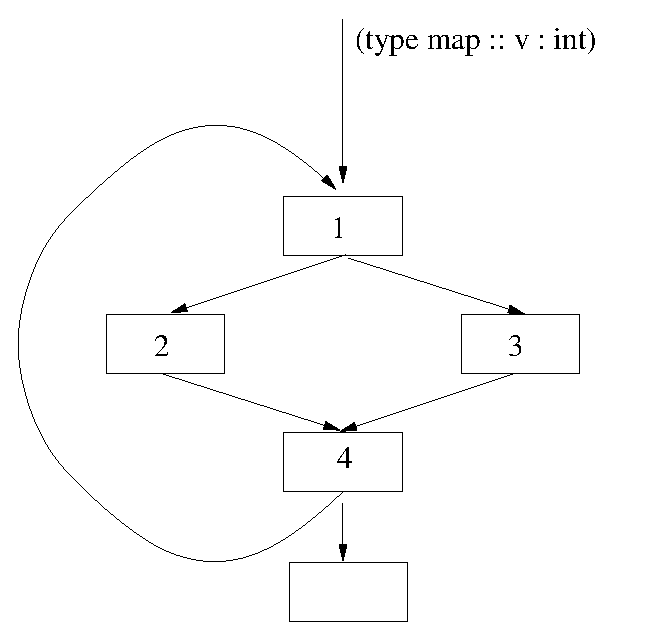
\includegraphics{Figs/4.1.eps}
  }
  \end{figure}
}
\frame
{
  \frametitle{\subsecname}
  \begin{figure}[h]
  \centering
  \scalebox{0.45}{
    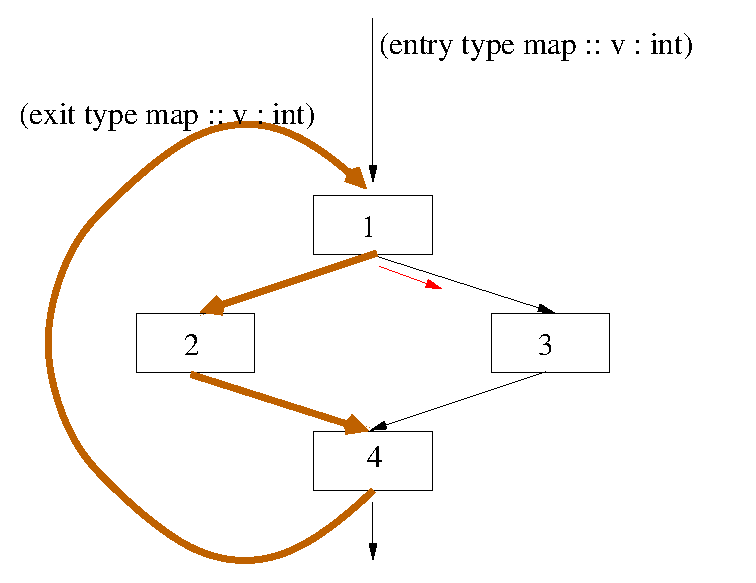
\includegraphics{Figs/4.2.eps}
  }
  \end{figure}
}
\frame
{
  \frametitle{\subsecname}
  \begin{figure}[h]
  \centering
  \scalebox{0.45}{
    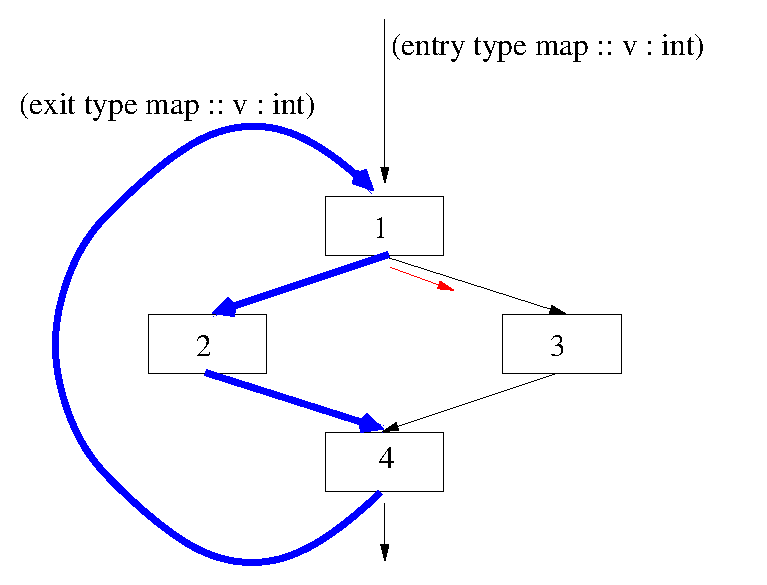
\includegraphics{Figs/4.3.eps}
  }
  \end{figure}
}
\subsection{Trace Tree Extension}
\frame
{
  \frametitle{\subsecname}
  \begin{figure}[h]
  \centering
  \scalebox{0.45}{
    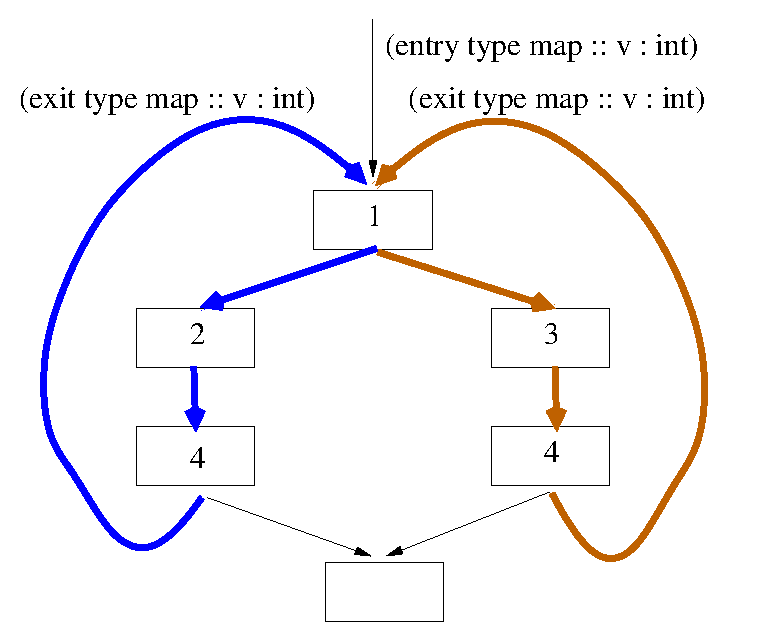
\includegraphics{Figs/4.4.eps}
  }
  \end{figure}
Note: Current Implementation extends only if 
        \begin{itemize}
          \item side exit is for control flow branch
          \item does not leave the loop
        \end{itemize}
}
\subsection{Problems with extension on return}
\frame
{
  \frametitle{\subsecname}
  \begin{figure}[h]
  \centering
  \scalebox{0.45}{
    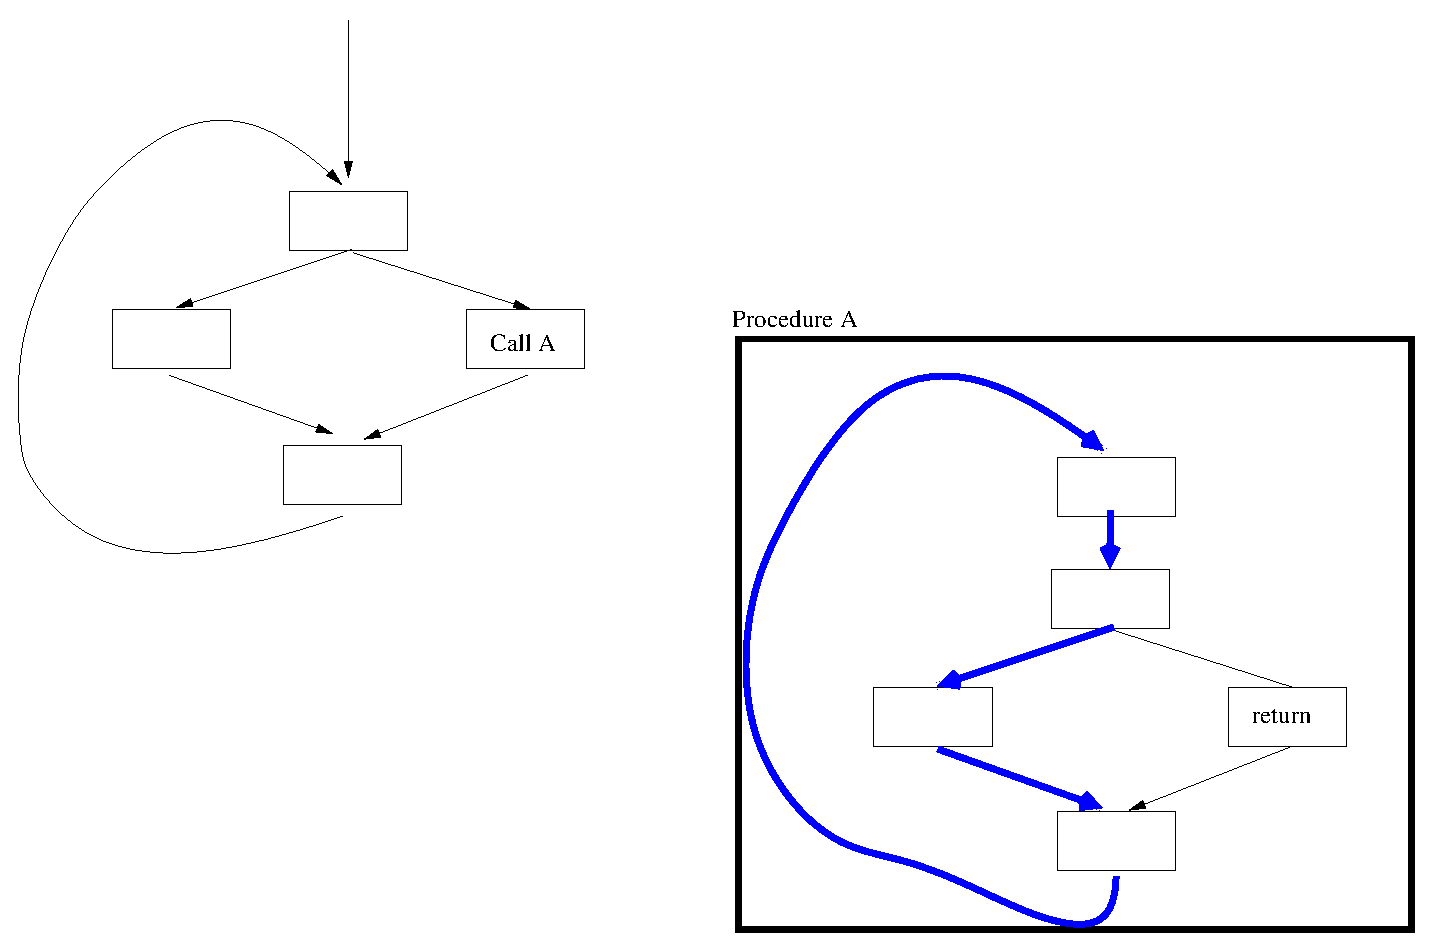
\includegraphics{Figs/4.4.1.eps}
  }
  \end{figure}
}
\subsection{Type Unstable Trace Handling}
\frame
{
  \frametitle{\subsecname}
  \begin{figure}[h]
  \centering
  \scalebox{0.45}{
    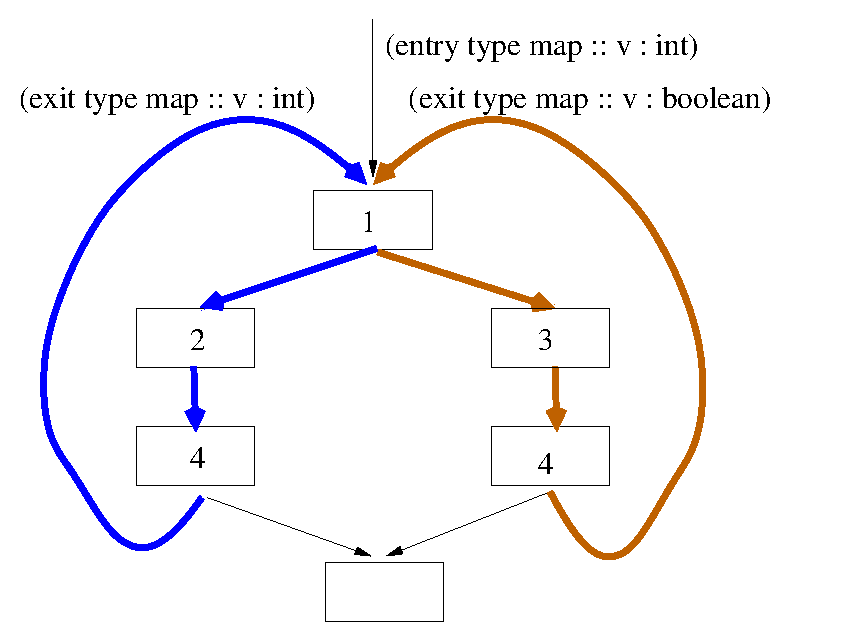
\includegraphics{Figs/4.5.eps}
  }
  \end{figure}
}
\frame
{
  \frametitle{\subsecname}
  \begin{figure}[h]
  \centering
  \scalebox{0.45}{
    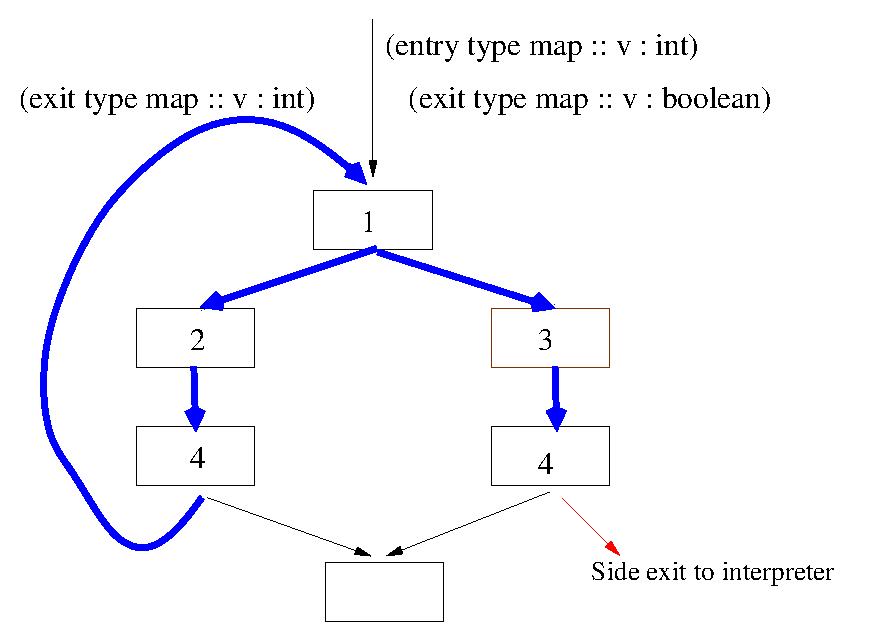
\includegraphics{Figs/4.5.1.eps}
  }
  \end{figure}
}
\frame
{
  \frametitle{\subsecname}
  \begin{figure}[h]
  \centering
  \scalebox{0.45}{
    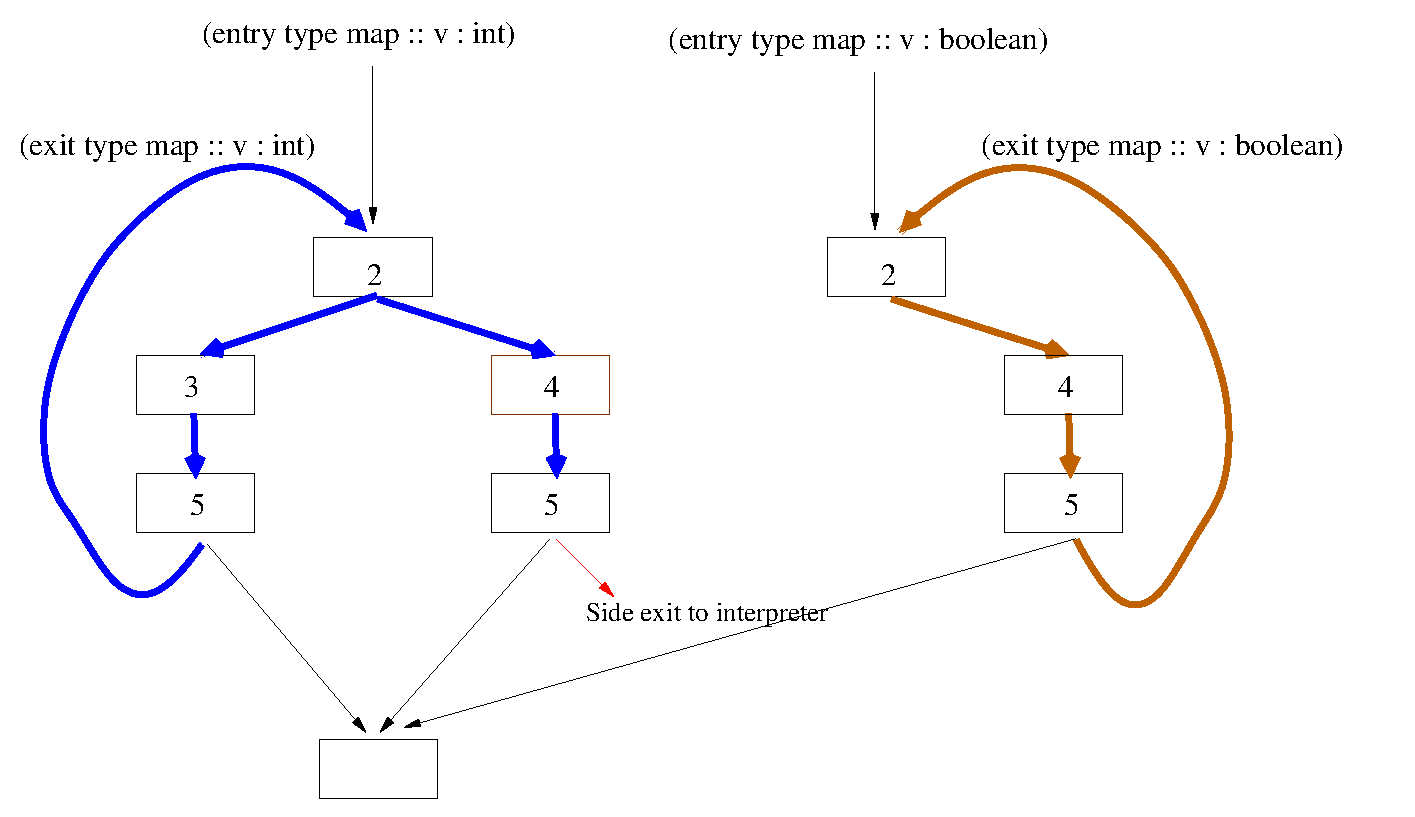
\includegraphics{Figs/4.6.eps}
  }
  \end{figure}
}
\frame
{
  \frametitle{\subsecname}
  \begin{figure}[h]
  \centering
  \scalebox{0.45}{
    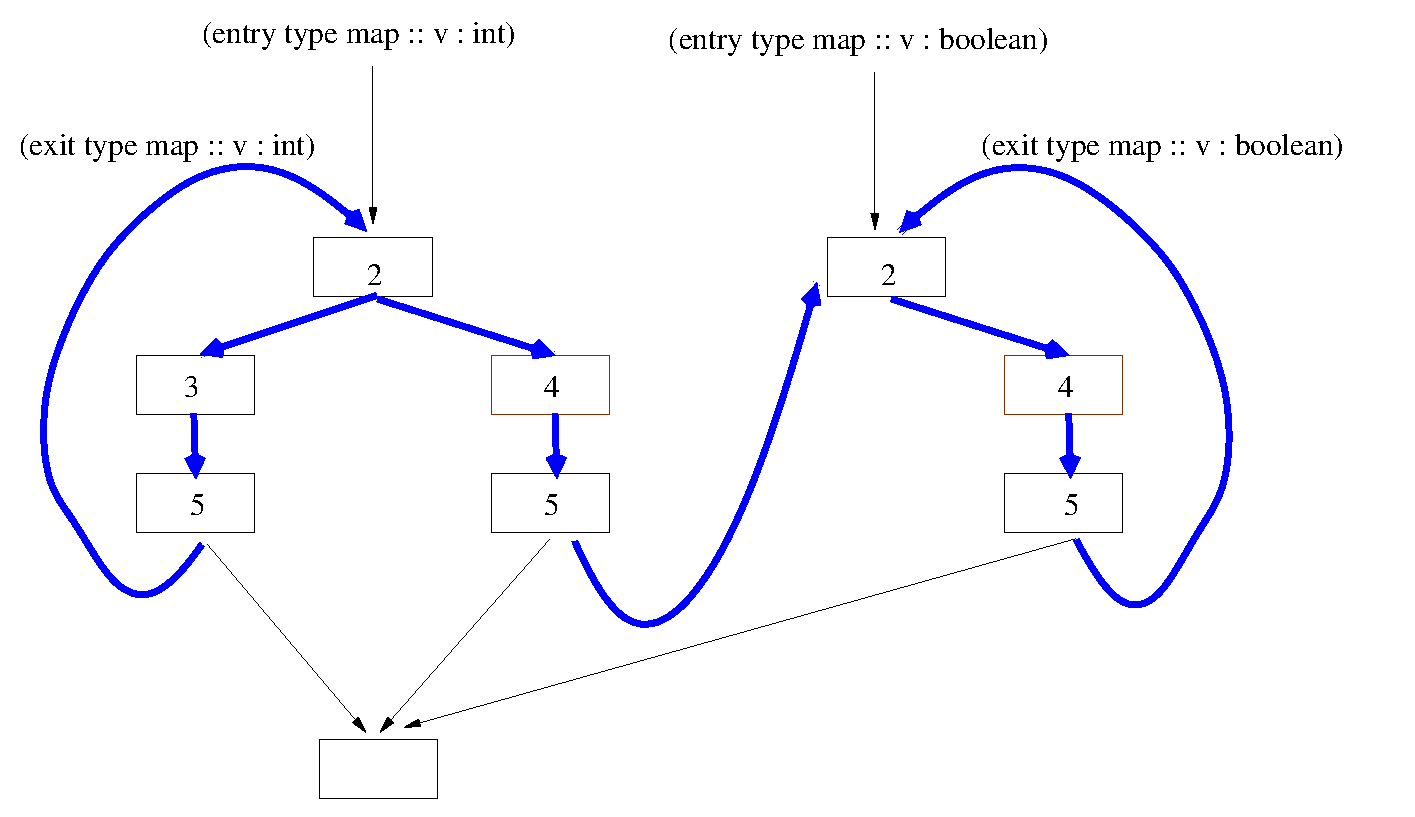
\includegraphics{Figs/4.7.eps}
  }
  \end{figure}
}
\section{Nested Trace Tree Formation}
\frame
{
  \frametitle{\secname}
  \begin{figure}[h]
  \centering
  \scalebox{0.45}{
    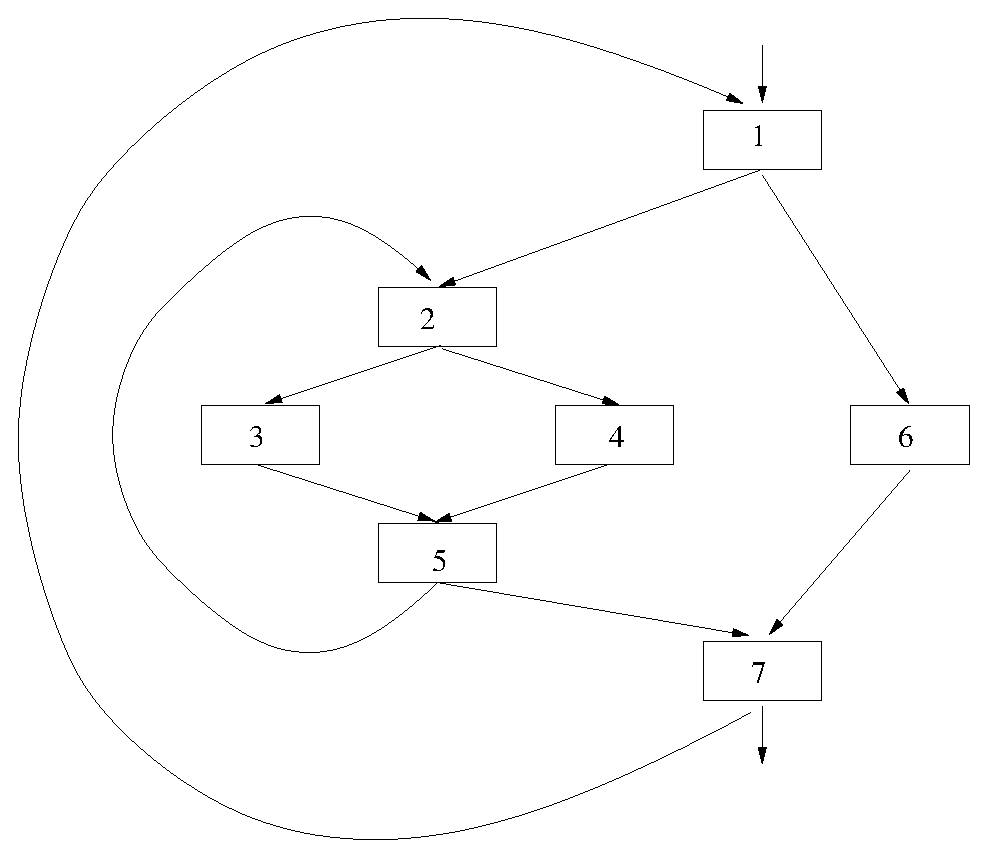
\includegraphics{Figs/2.1.eps}
  }
  \end{figure}

  
}
\frame
{
  \frametitle{\secname}
  \begin{figure}[h]
  \centering
  \scalebox{0.45}{
    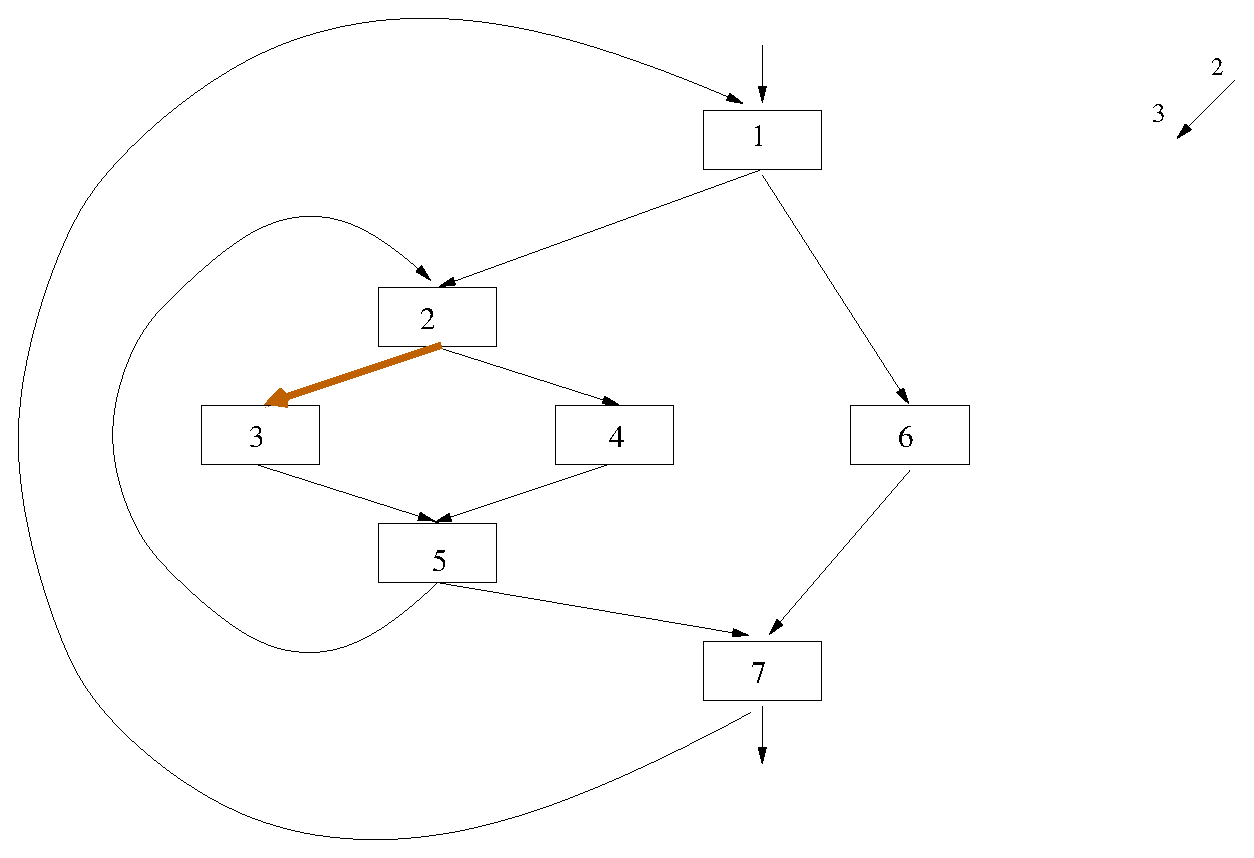
\includegraphics{Figs/2.2.eps}
  }
  \end{figure}
}
\frame
{
  \frametitle{\secname}
  \begin{figure}[h]
  \centering
  \scalebox{0.45}{
    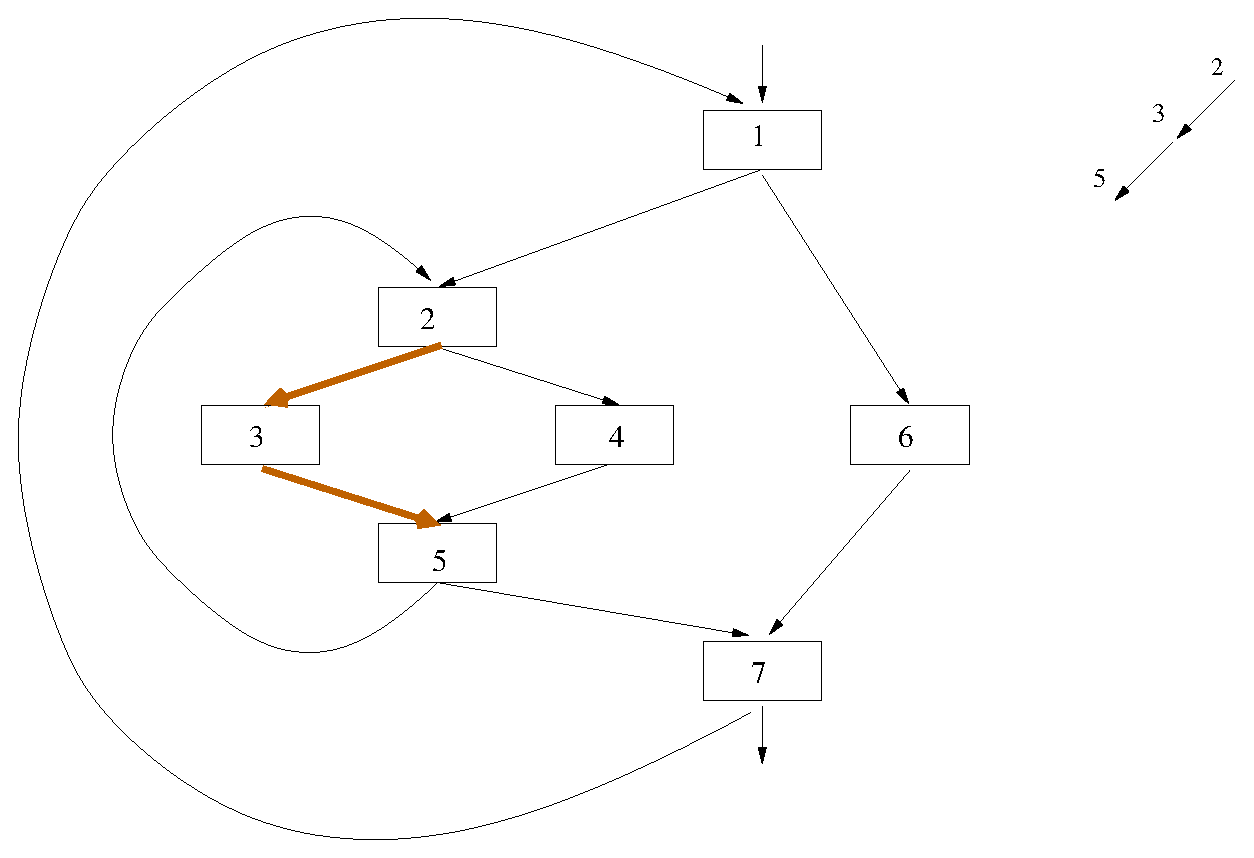
\includegraphics{Figs/2.3.eps}
  }
  \end{figure}
}
\frame
{
  \frametitle{\secname}
  \begin{figure}[h]
  \centering
  \scalebox{0.45}{
    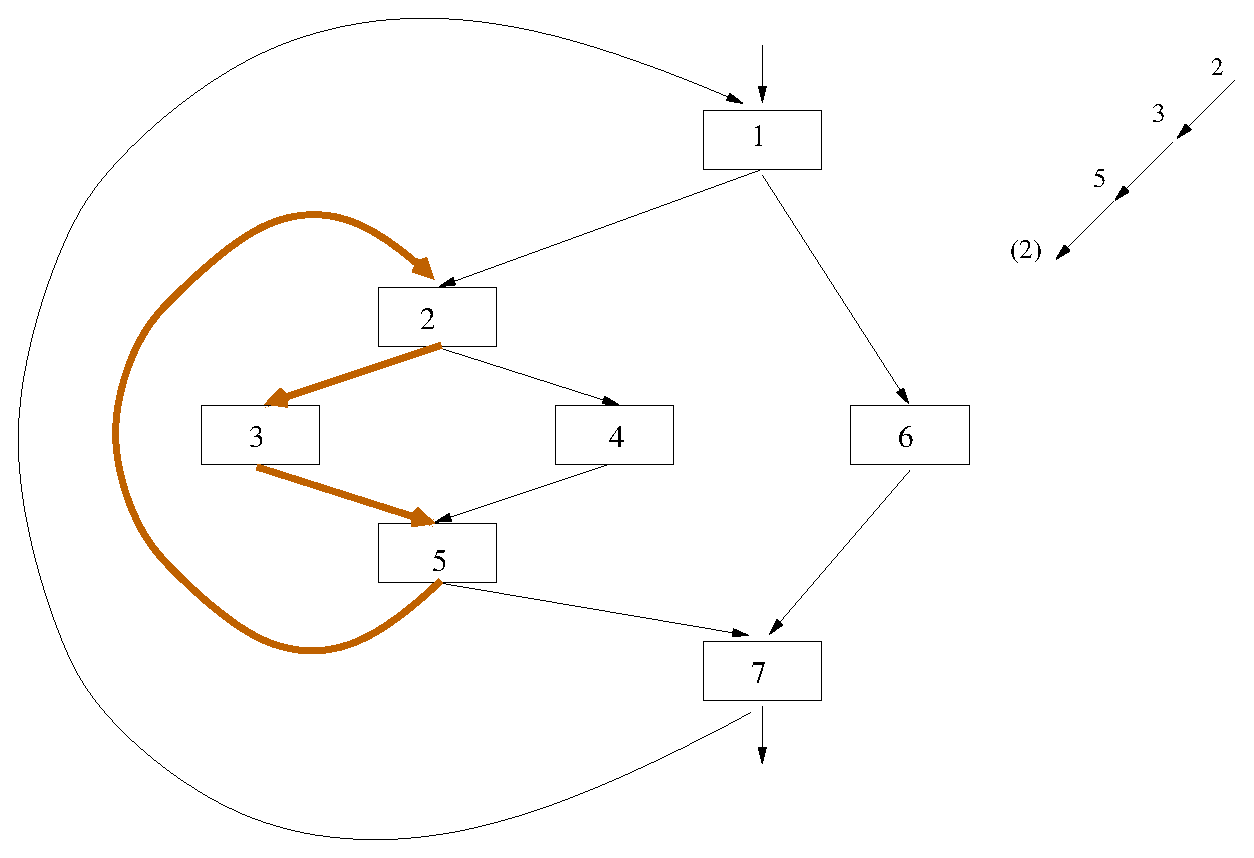
\includegraphics{Figs/2.4.eps}
  }
  \end{figure}
}
\frame
{
  \frametitle{\secname}
  \begin{figure}[h]
  \centering
  \scalebox{0.45}{
    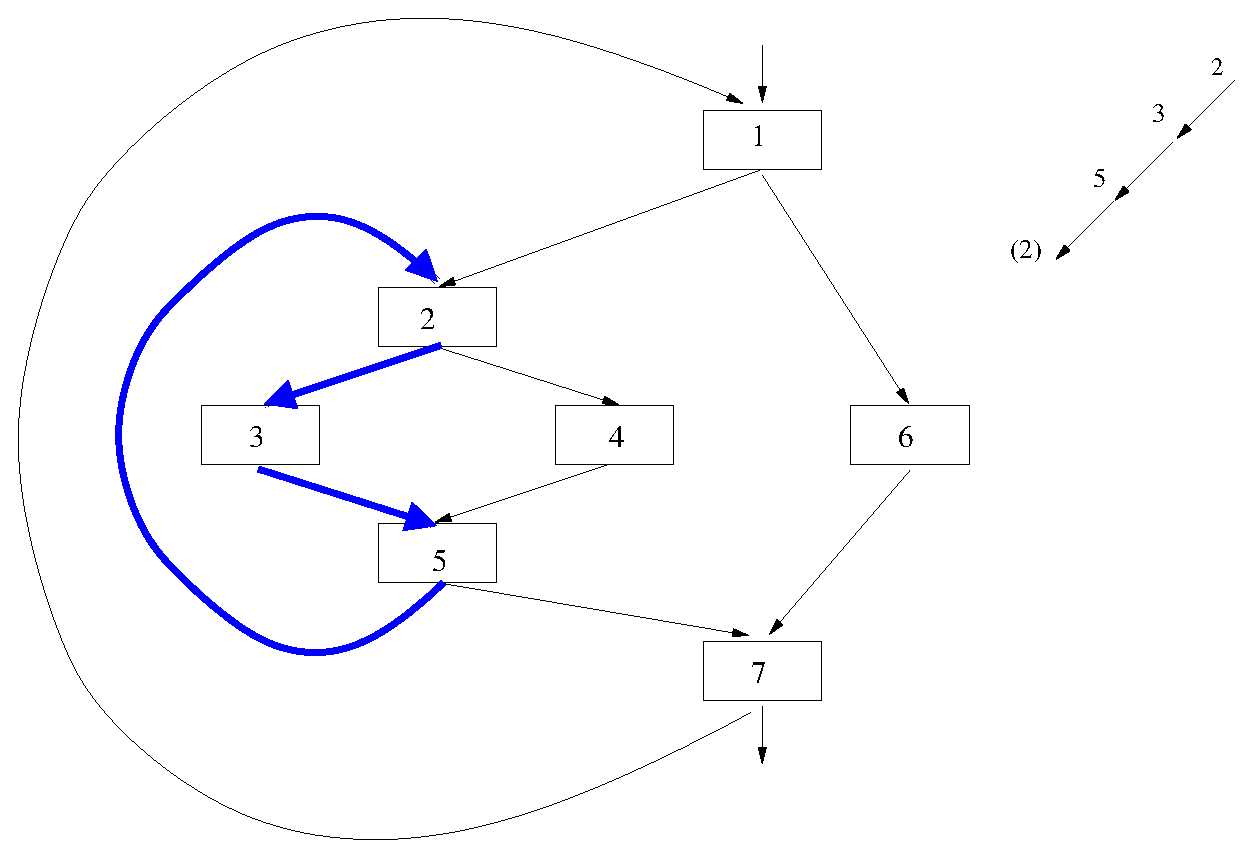
\includegraphics{Figs/2.4.1.eps}
  }
  \end{figure}
}
\subsection{Continue tracing for outer loop}
\frame
{
  \frametitle{\subsecname}
  \begin{figure}[h]
  \centering
  \scalebox{0.45}{
    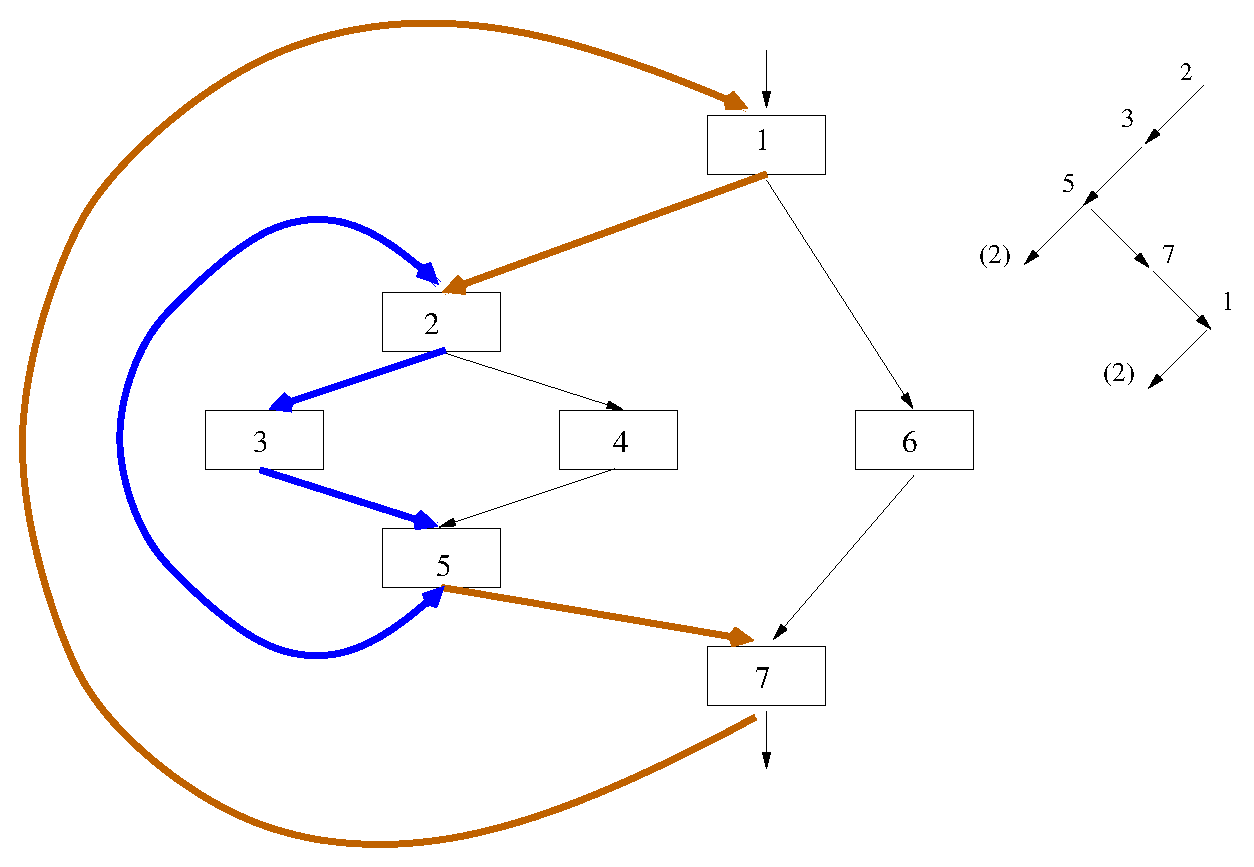
\includegraphics{Figs/2.5.eps}
  }
  \end{figure}
}
\frame
{
  \begin{figure}[h]
  \centering
  \scalebox{0.45}{
    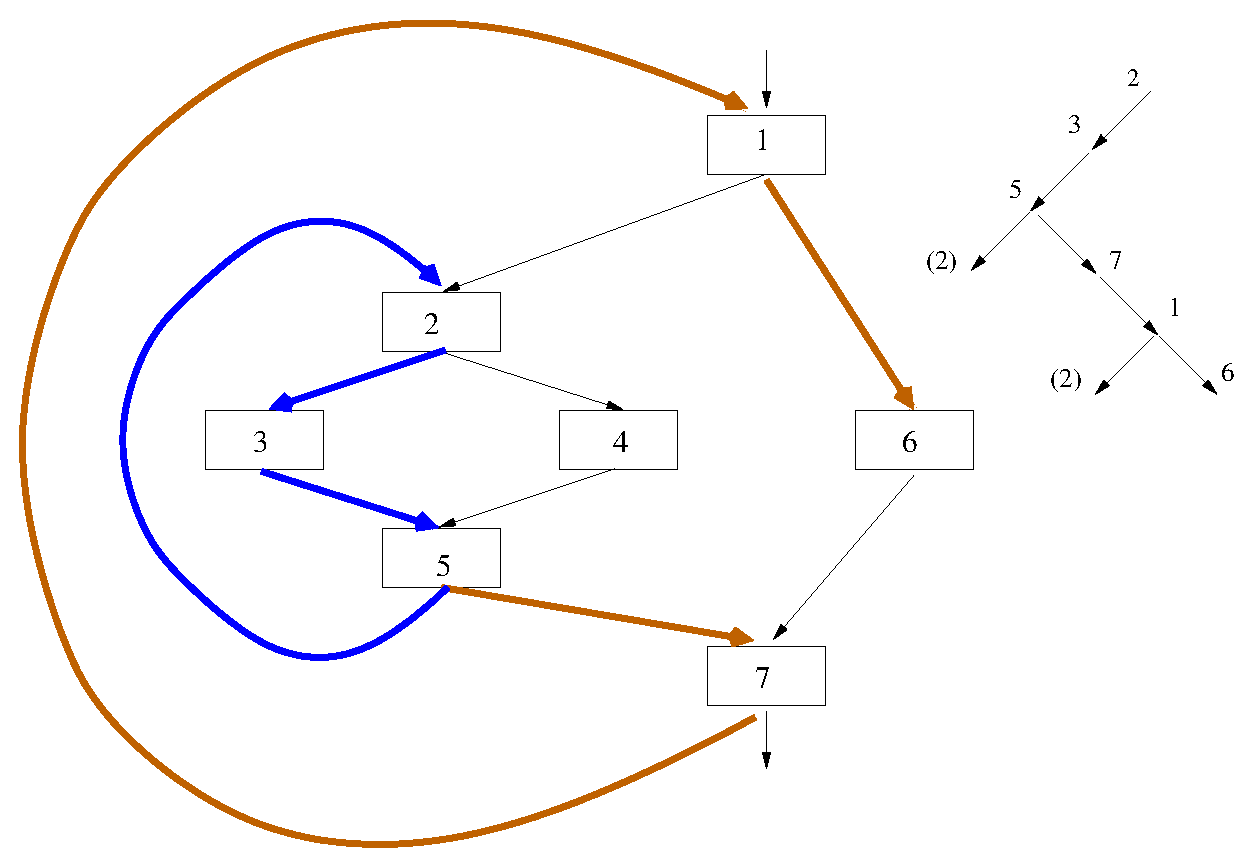
\includegraphics{Figs/2.7.eps}
  }
  \end{figure}
}
\frame
{
  \frametitle{\subsecname}
  \begin{figure}[h]
  \centering
  \scalebox{0.45}{
    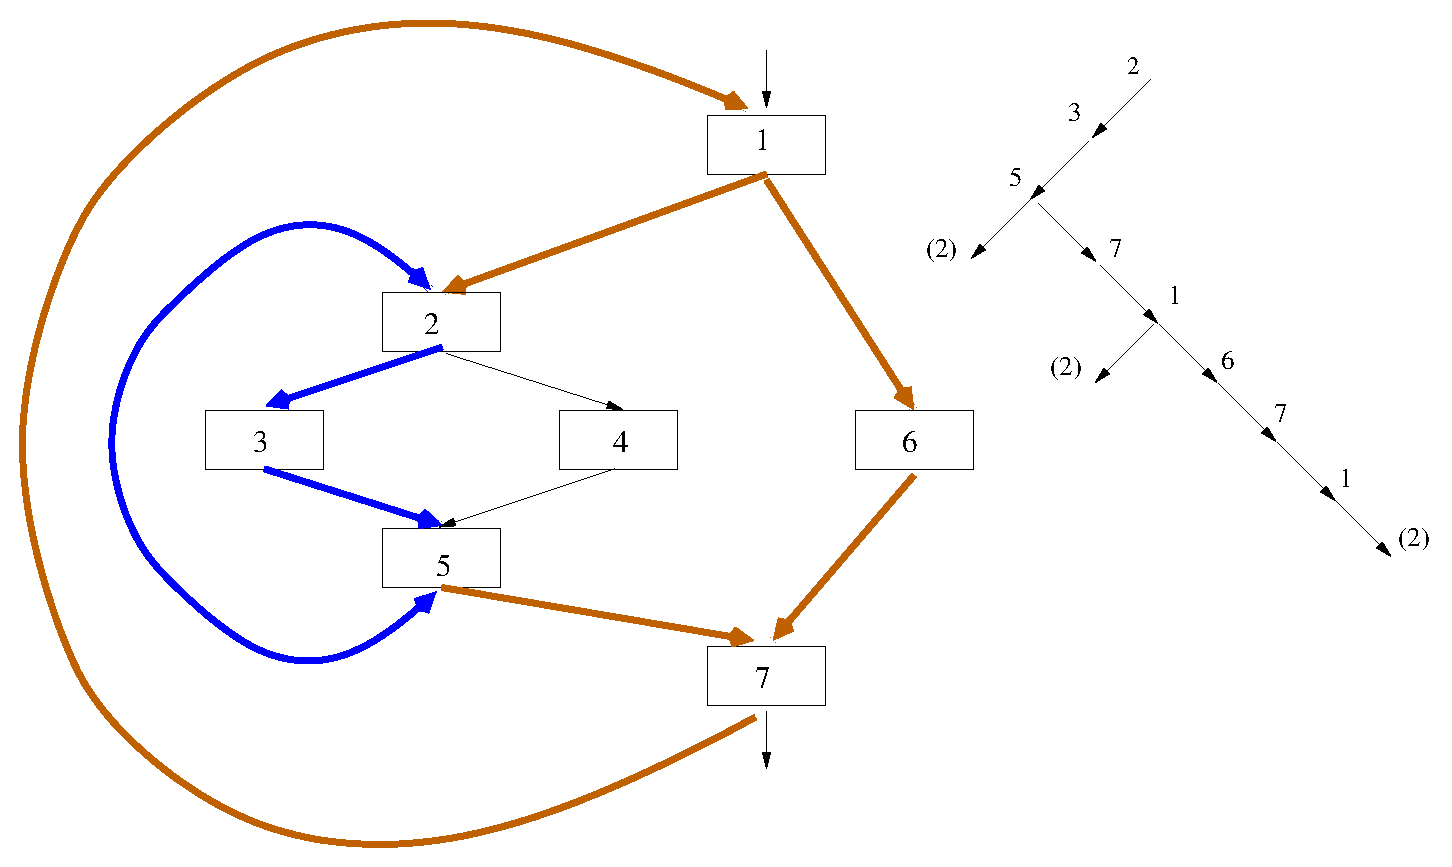
\includegraphics{Figs/2.8.eps}
  }
  \end{figure}
}
\frame
{
  \frametitle{\subsecname}
  \begin{figure}[h]
  \centering
  \scalebox{0.45}{
    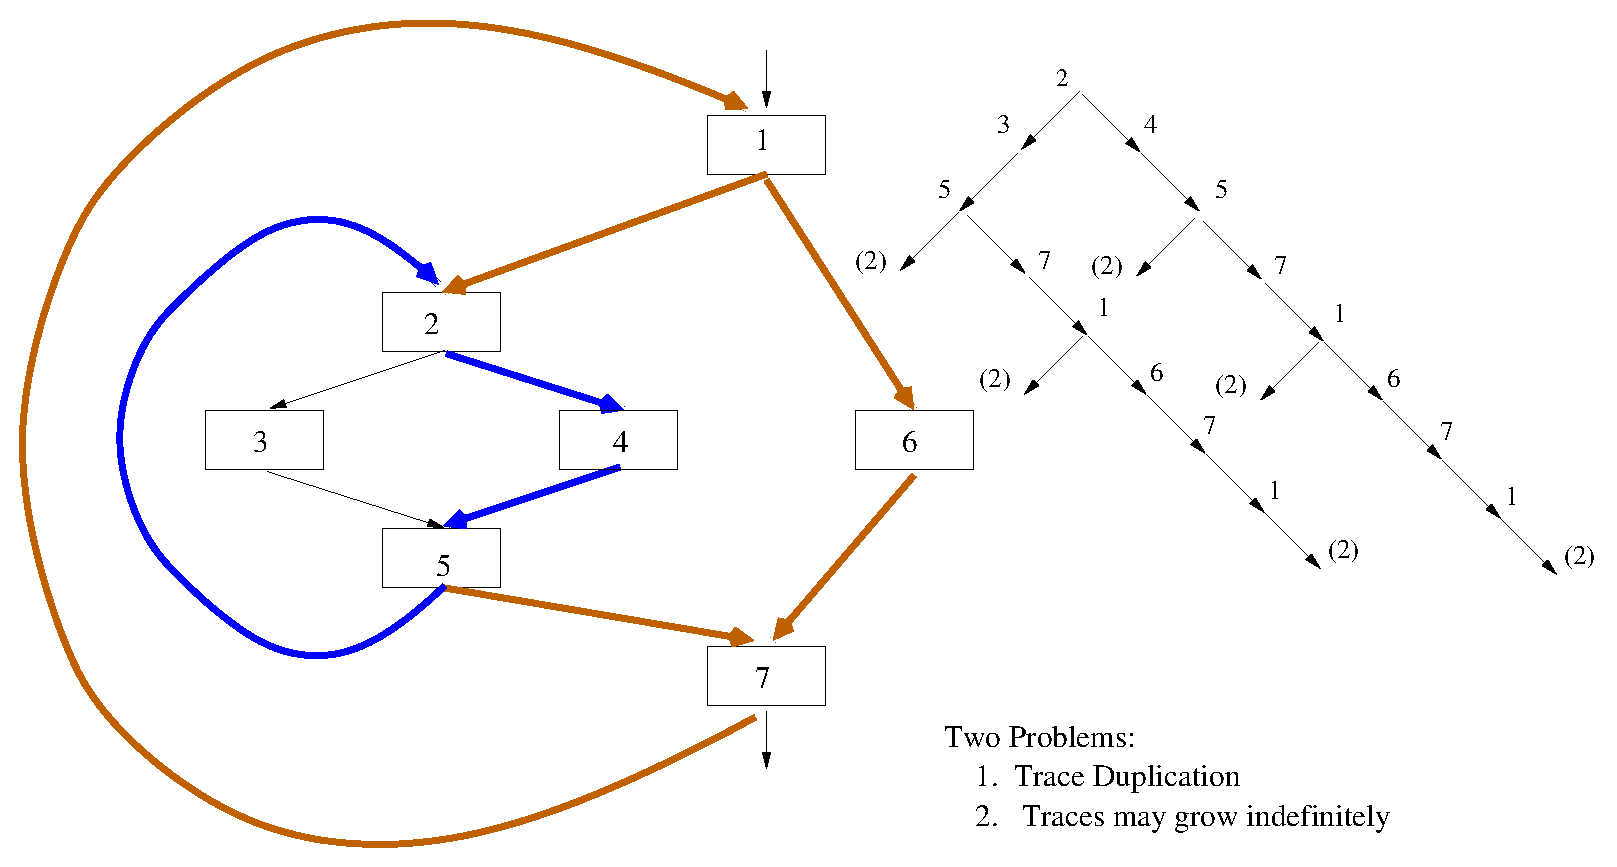
\includegraphics{Figs/2.9.eps}
  }
  \end{figure}

}

\subsection{Separate traces}
\frame
{
  \frametitle{\subsecname}
  \begin{figure}[h]
  \centering
  \scalebox{0.45}{
    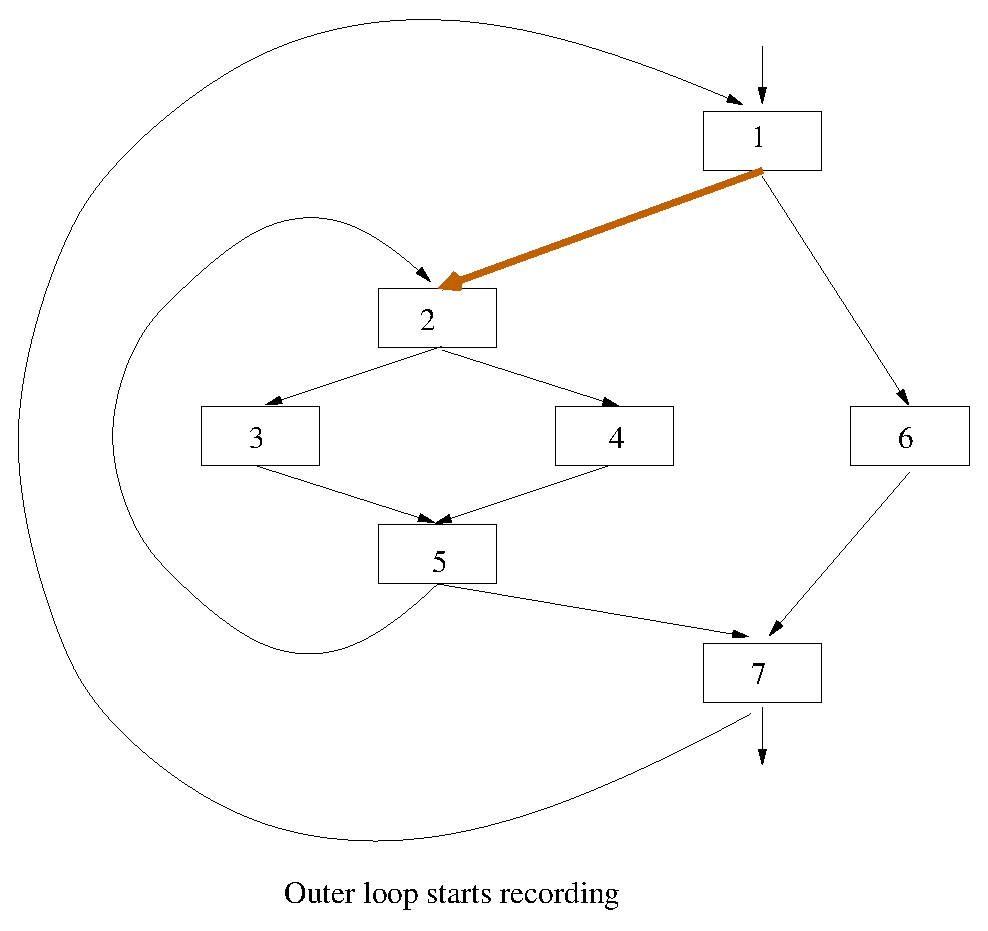
\includegraphics{Figs/3.1.eps}
  }
  \end{figure}
}
\frame
{
  \frametitle{\subsecname}
  \begin{figure}[h]
  \centering
  \scalebox{0.45}{
    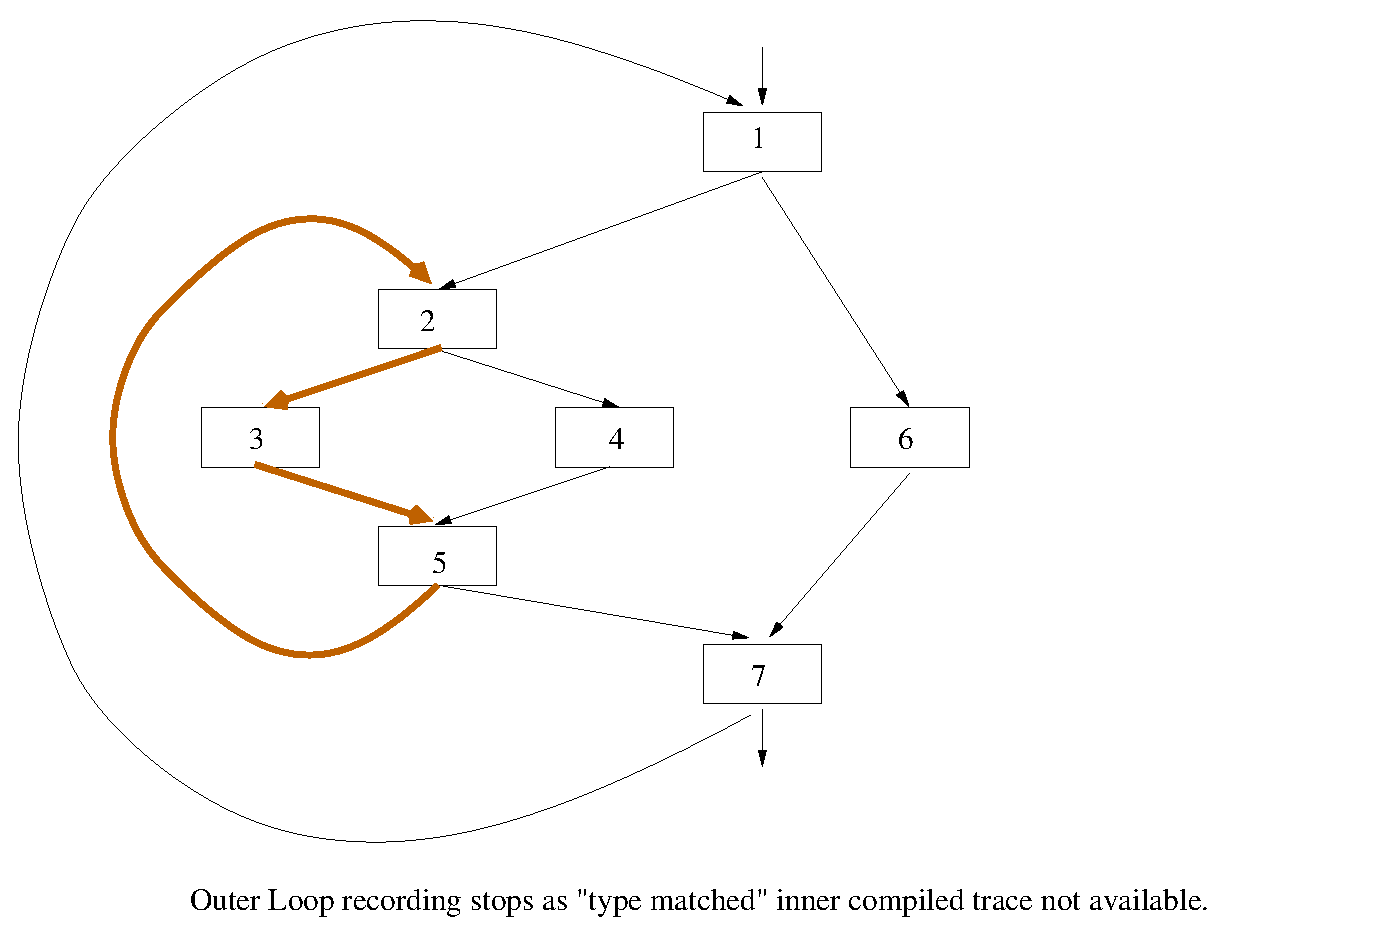
\includegraphics{Figs/3.2.eps}
  }
  \end{figure}
}
\frame
{
  \frametitle{\subsecname}
  \begin{figure}[h]
  \centering
  \scalebox{0.45}{
    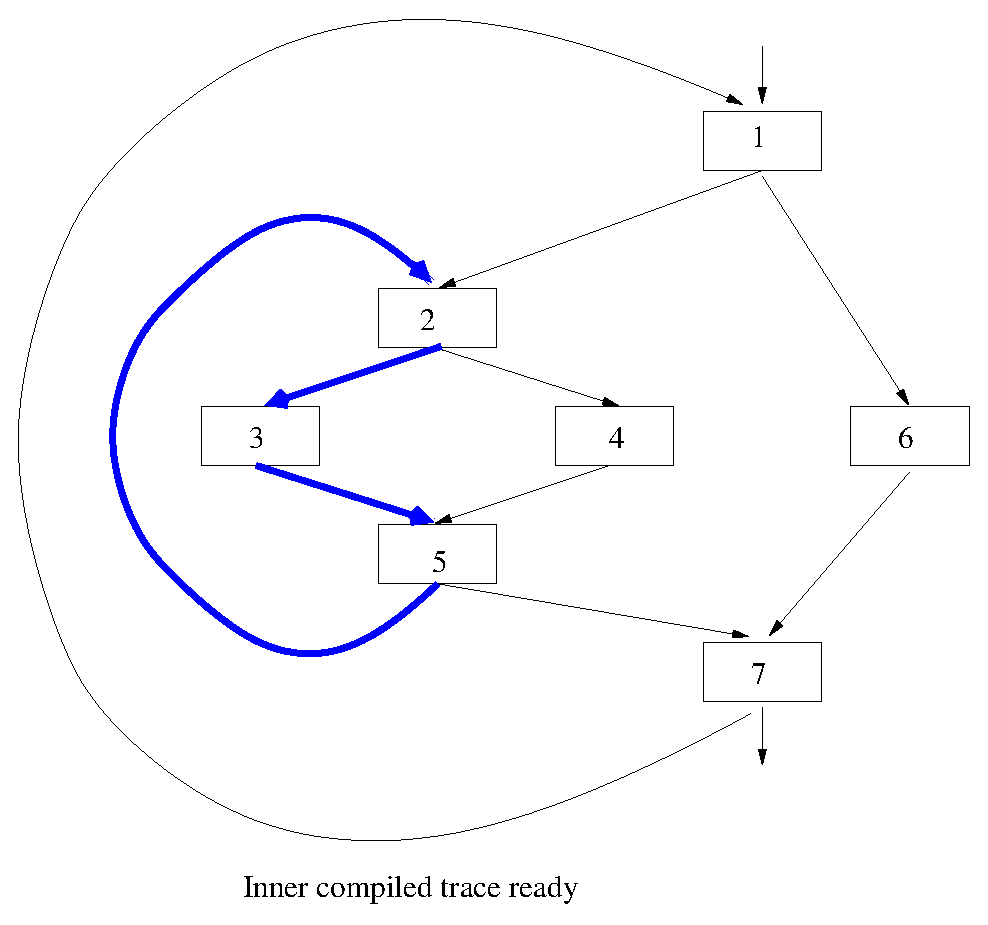
\includegraphics{Figs/3.3.eps}
  }
  \end{figure}
}
\frame
{
  \frametitle{\subsecname}
  \begin{figure}[h]
  \centering
  \scalebox{0.45}{
    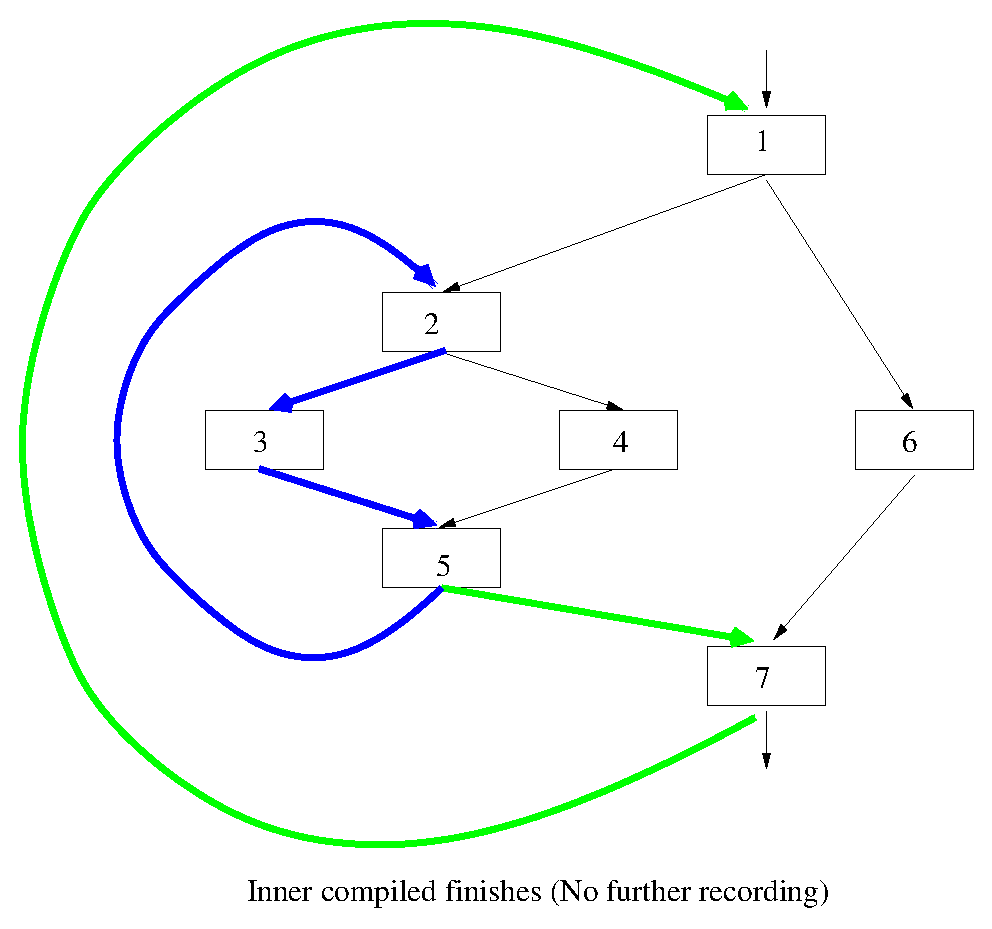
\includegraphics{Figs/3.3.1.eps}
  }
  \end{figure}
}
\frame
{
  \frametitle{\subsecname}
  \begin{figure}[h]
  \centering
  \scalebox{0.45}{
    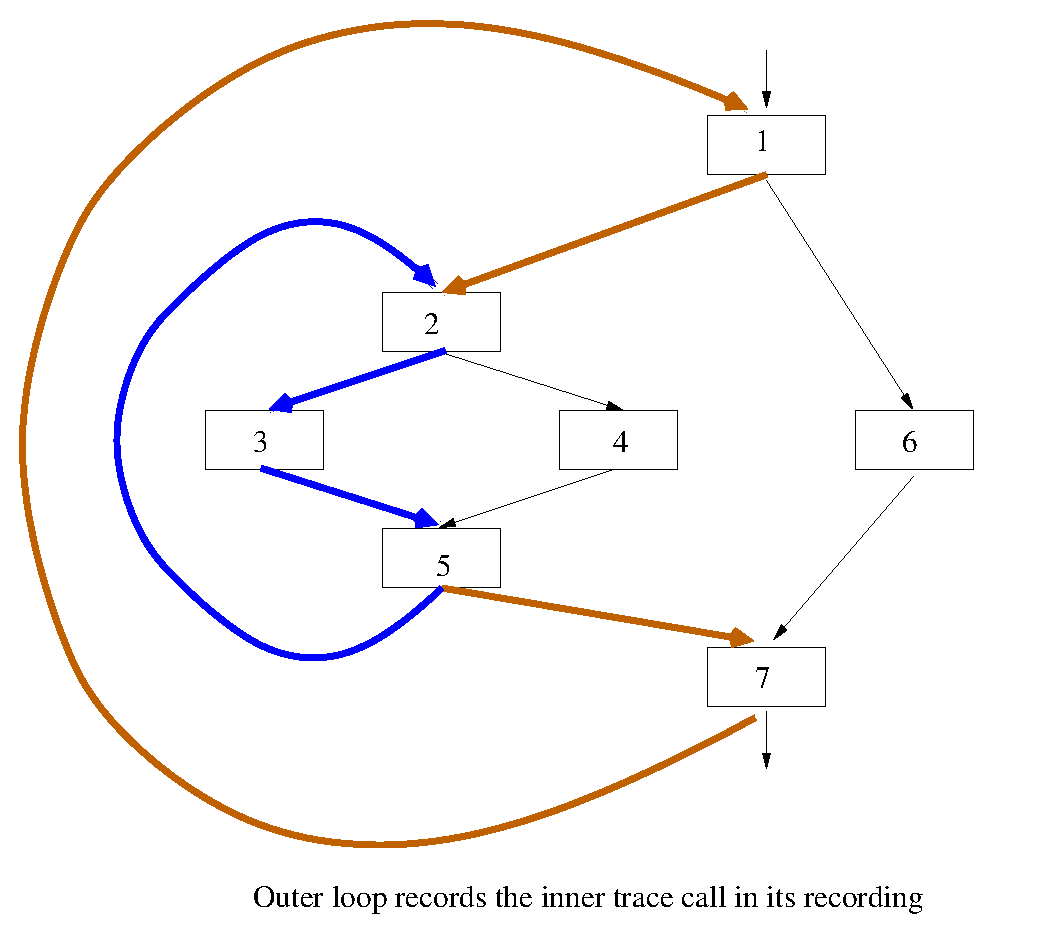
\includegraphics{Figs/3.4.eps}
  }
  \end{figure}
}

\cmt{
\frame
{
  \frametitle{\subsecname}
  \begin{figure}[h]
  \centering
  \scalebox{0.45}{
    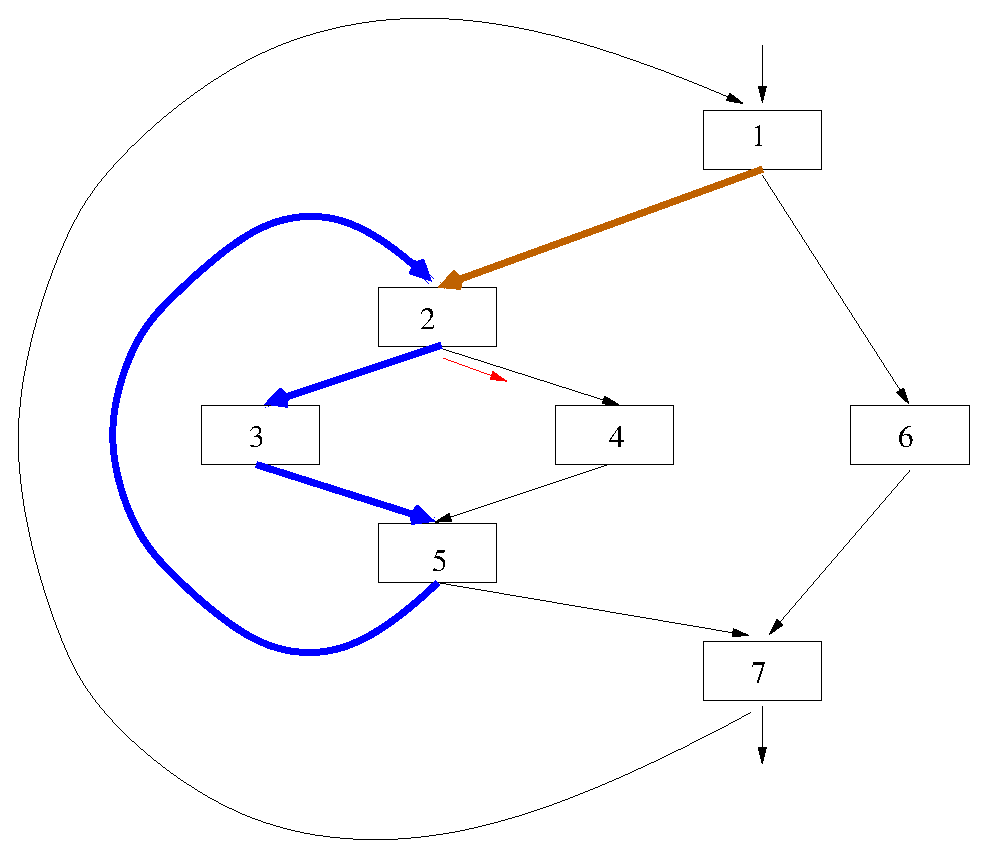
\includegraphics{Figs/3.4.1.eps}
  }
  \end{figure}
  What if during recording of outer loop, the inner trace got a side exit !!
}
\frame
{
  \frametitle{\subsecname}
  \begin{figure}[h]
  \centering
  \scalebox{0.45}{
    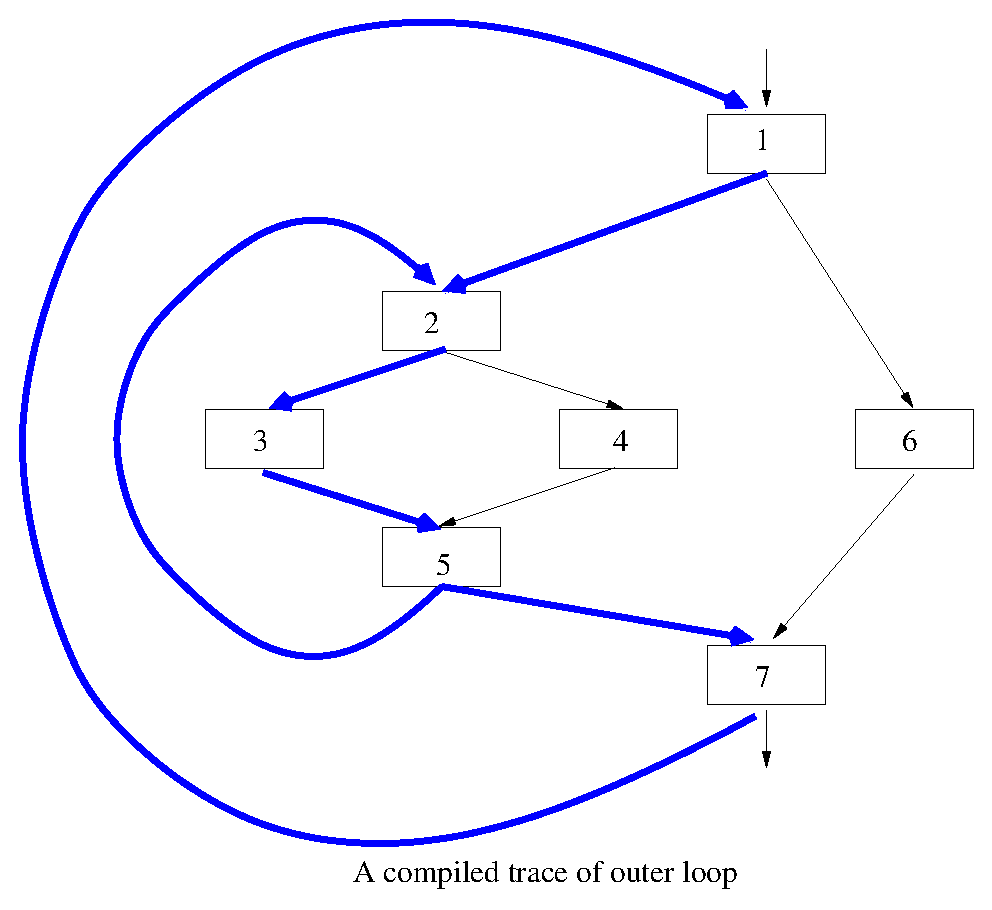
\includegraphics{Figs/3.5.eps}
  }
  \end{figure}
}
\frame
{
  \frametitle{\subsecname}
  \begin{figure}[h]
  \centering
  \scalebox{0.45}{
    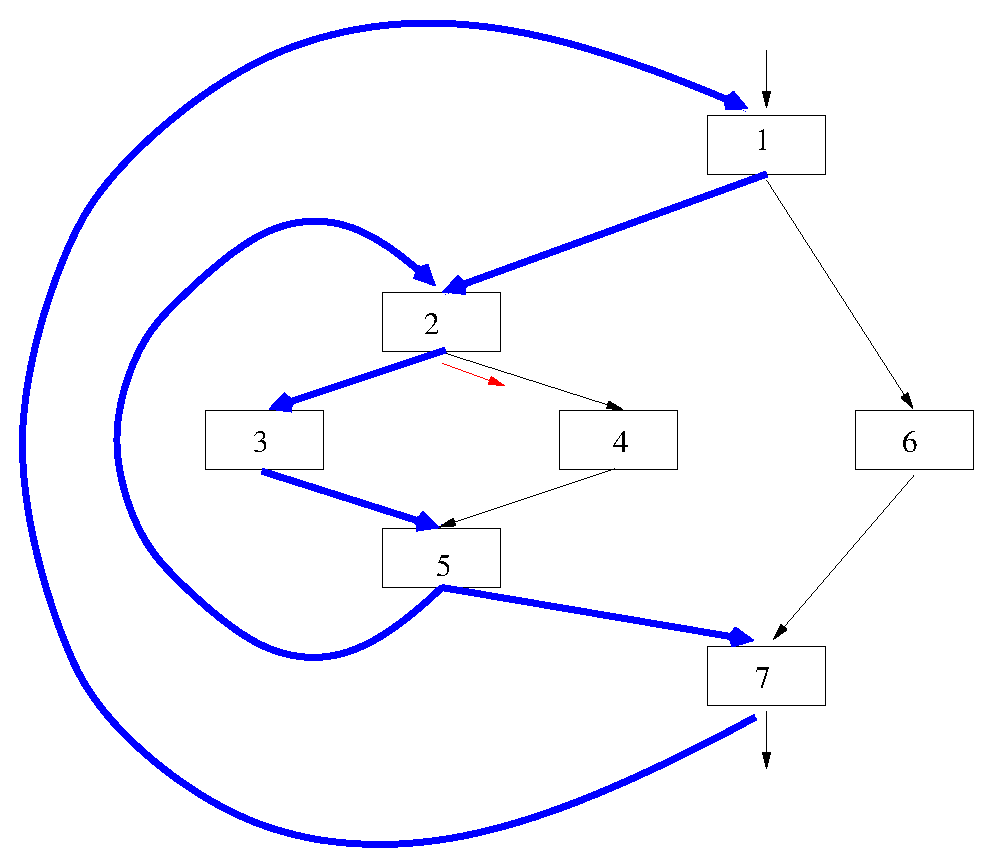
\includegraphics{Figs/3.5.1.eps}
  }
  \end{figure}

  What if during execution of outer loop, the inner trace got a side exit !!
}

}

\cmt{
\subsection{Blacklisting}
\frame
{
  \frametitle{\subsecname}
  \begin{itemize}
   \item What if a hot loop contain traces whose recording always fail ? 
   \item Solution : Blacklist with back-off on recording
   \end{itemize}
}
}
\cmt{recording overhead is huge.}

\cmt{
\subsection{Recording}
\frame
{
  \frametitle{\subsecname}
  \begin{itemize}
    \item While interpreting traces are recorded and transformed into LIR. WHY ?? 
      \begin{itemize}
        \item LIR traces are type specialized
        \item LIR traces are representation specialized w.r.t objects
        \item LIR traces are representation specialized w.r.t numbers
        \item LIR traces inline functions
      \end{itemize}  
    \item All the above LIR features need guards
  \end{itemize}  
}
}

\section{Trace  Optimization}
\subsection{Trace Tree Optimization}
\frame
{
  \frametitle{\subsecname}
  \begin{itemize}
    \item Optimization Goal: Make compilation fast. (Done by NanoJIT)
    %\begin{itemize}
      %\item Restrict to small set of optimization
      %\uncover<3> {  \item Avoid any reordering optimizations } 
     % \item leverage the fact that the LIR is in SSA form 
    %\end{itemize}
    \item Optimizations are performed in 2 phases: forward and backward 
  \end{itemize}     
}

\subsection{Forward Optimizations}
\frame
{
  \frametitle{\subsecname}
  \begin{itemize}
    \item While recording on each instruction basis.
      \begin{itemize}
        \item Constant subexpression elimination
        \item Expression simplification and algebraic identities
      \end{itemize}  
  \end{itemize}  
}
\subsection{Backward optimizations}
\frame
{
  \frametitle{\subsecname}
  \begin{itemize}
    \item When recording is complete.
    \begin{itemize}
      \item dead data-stack store elimination
      \item dead call-stack store elimination
      \item dead code elimination
    \end{itemize}  
  \end{itemize}    
}

\subsection{Register Allocation}
\frame
{
  \frametitle{\subsecname}
  \begin{figure}[h]
  \centering
  \scalebox{0.45}{
    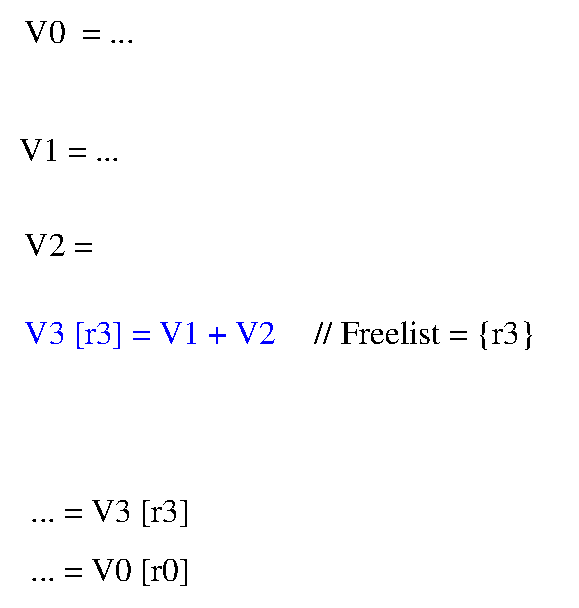
\includegraphics{Figs/5.4.eps}
  }
  \end{figure}
}
\subsection{Register Allocation}
\frame
{
  \frametitle{\subsecname}
  \begin{figure}[h]
  \centering
  \scalebox{0.45}{
    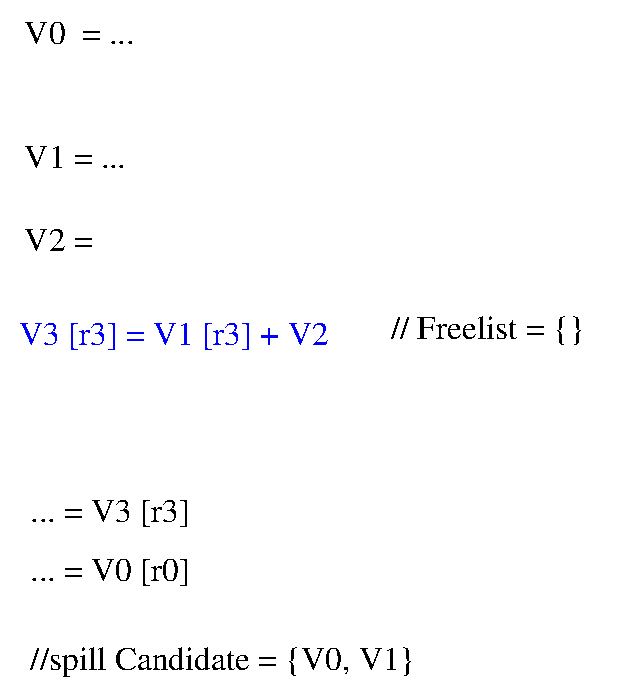
\includegraphics{Figs/5.2.eps}
  }
  \end{figure}
}
\subsection{Register Allocation}
\frame
{
  \frametitle{\subsecname}
  \begin{figure}[h]
  \centering
  \scalebox{0.45}{
    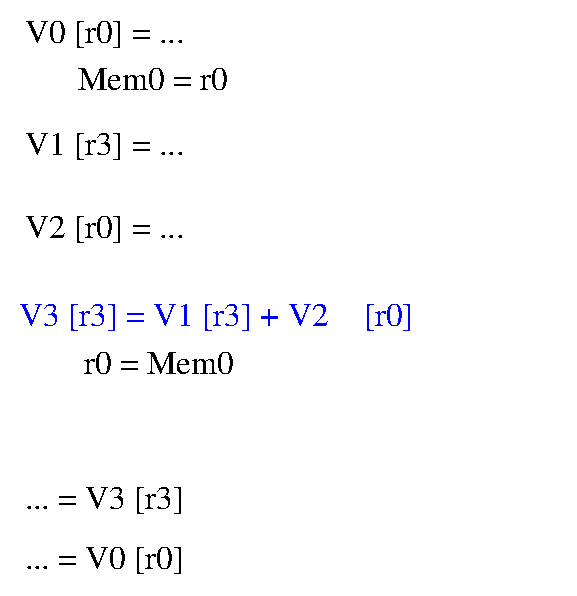
\includegraphics{Figs/5.3.eps}
  }
  \end{figure}
}

\section{Evaluation}
\subsection{Setup}
\frame
{
  \frametitle{\subsecname}
  \begin{itemize}
    \item SunSpider Benchmark suite is used
    \begin{itemize}
        \item SpiderMonkey: JS interpreter. \textbf{Baseline for comparison}
        \item TraceMonkey: The proposed compilation strategy
        \item SquirrelFish Extreme (SFX)
                                          \cmt{
        : Call threaded JS interpreter
                                          }
        \item V8, Javascript VM from Google
          \cmt{
            : Method compiling JS VM
          }
    \end{itemize}
  \end{itemize}
}
\subsection{Results}
\frame
{
  \frametitle{\subsecname}
  \begin{itemize}
    \item Speedup (TraceMonkey) spreads between 0.9 and 25. 
    \item Performance depends on
    \begin{itemize}
      \item Fraction of bytecode executed as native trace
      \item Cost of Recording, Compilation, Calling Traces
      \cmt{good perf when where VM spends majority of time running native code}
    \end{itemize}
    \item Outperform both the VMs on 9/26 benchmarks.
  \end{itemize}
}

\subsection{My Critique}
\frame
{
  \frametitle{\subsecname}
  \begin{itemize}
    \item Novel approach. 
    \item Entirely loop based. 
    \item Sunspider is too small a benchmark to show the effectiveness.
    \cmt{
      This method will works if there exist long trip count loops in the program, which is not
usual in real web pages ... it is mostly method driven... but these will be help ful in
online gaming or google maps which do have long loops
    }
  \end{itemize}
}

\section{Questions?}
\subsection{Questions?}
\frame
{}

\subsection{Static Type Inferencing}
\frame
{
  \frametitle{\subsecname}
  \begin{figure}[h]
  \centering
  \scalebox{0.45}{
    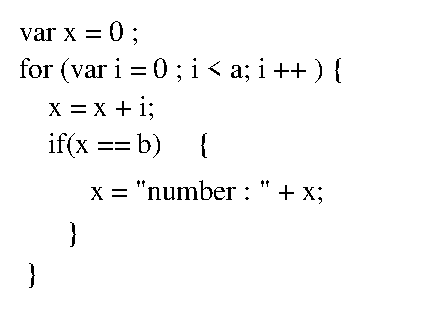
\includegraphics{Figs/10.eps}
  }
  \end{figure}
}

\subsection{Speedup Comparison}
\frame
{
  \frametitle{\subsecname}
  \begin{figure}[h]
  \centering
  \scalebox{0.45}{
    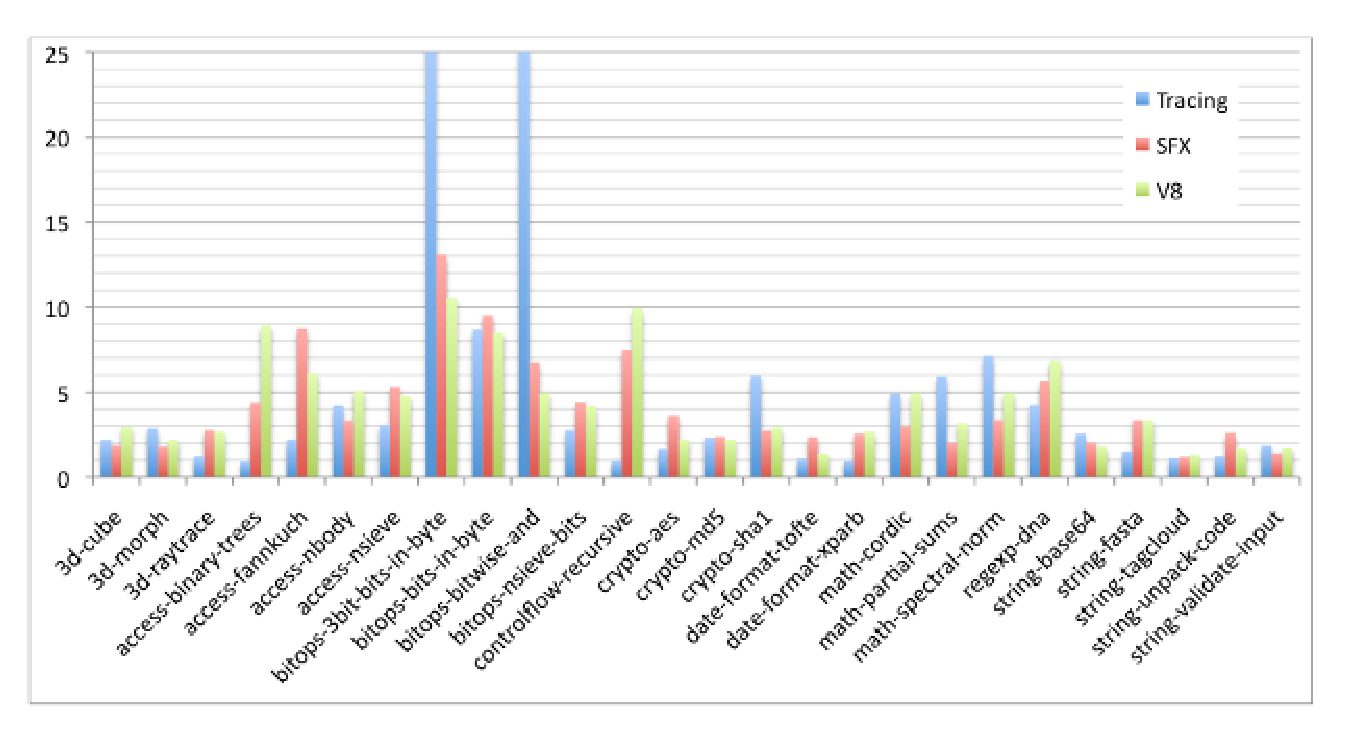
\includegraphics{Figs/6.eps}
  }
  \end{figure}
  [Figure copied from presentation paper]
}
\subsection{Fraction of time spend in major VM activities}
\frame
{
  \frametitle{\subsecname}
  \begin{figure}[h]
  \centering
  \scalebox{0.45}{
    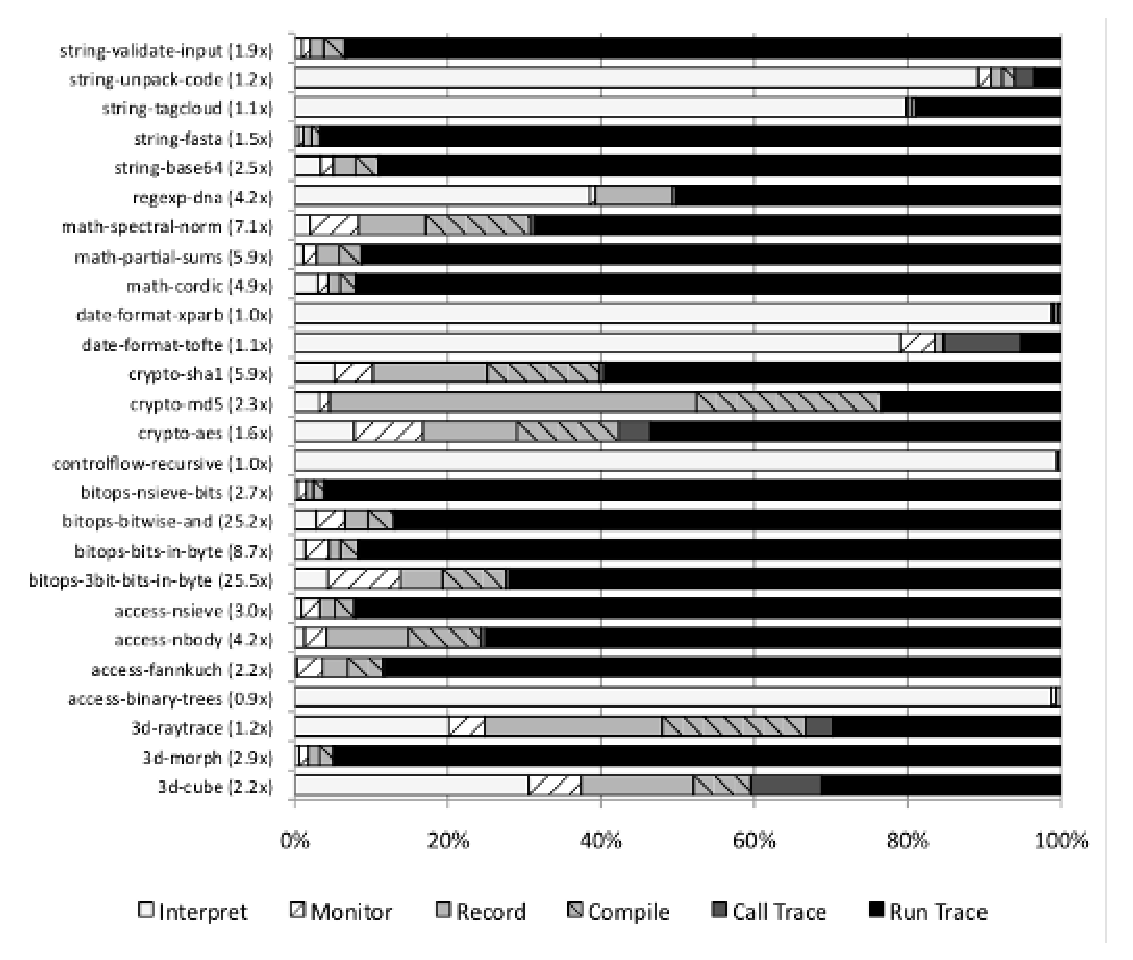
\includegraphics{Figs/7.eps}
  }
  \end{figure}
  [Figure copied from presentation paper]
}

\subsection{Trace recording statistics for Sunspider Benchmark}
\frame
{
  \frametitle{\subsecname}
  \begin{figure}[h]
  \centering
  \scalebox{0.45}{
    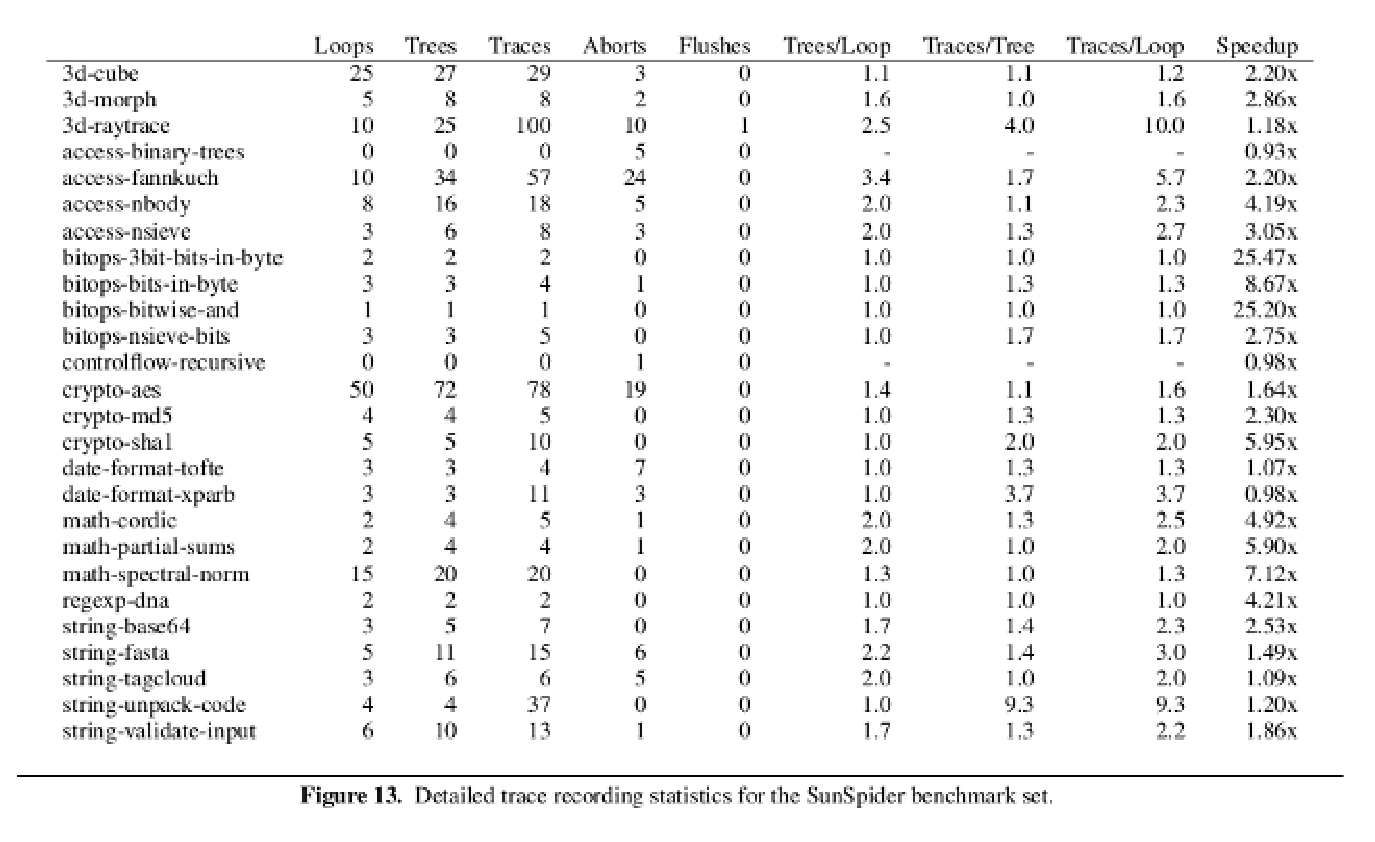
\includegraphics{Figs/8.eps}
  }
  \end{figure}
  [Figure copied from presentation paper]
}

\subsection{Results Continued}
\frame
{
  \frametitle{\subsecname}
  \begin{itemize}
    \item Overall performance speedup of native trace execution  = $\frac{\text{Time per bytecode execution in Interpreter}}{\text{Time per bytecode execution in native code}  } = 3.9$
      \cmt{
    \item Native trace takes 9 cycles/ byte code as compared to the interpreter ( 35 cycle/ bytecode) 
      }
    \item Other VMs have an overall performance speedup of 3.0
    \item TraceMonkey recording \& compilation 200 times slower than interpreter speed.
  \end{itemize}
}

\subsection{When recording aborts}
\frame
{
  \frametitle{\subsecname}
  \begin{itemize}
    \item Type unstable loop.
    \item Trace length exceeds a threashold.
    \item Outer loop recording finds an uncompiled inner trace.
  \end{itemize}  
}

\subsection{Types in C Vs JS}
\frame
{
  \frametitle{\subsecname}
  \begin{figure}[h]
  \centering
  \scalebox{0.45}{
    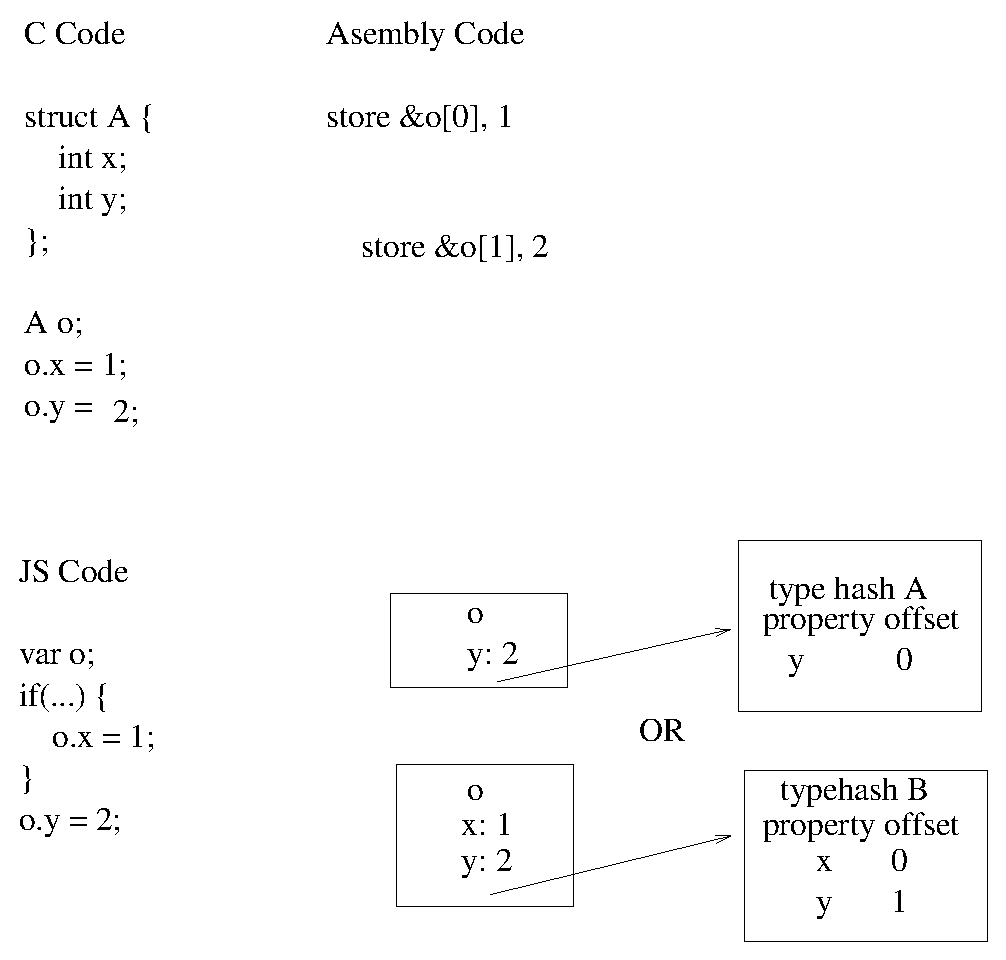
\includegraphics{Figs/11.eps}
  }
  \end{figure}
}


\subsection{NanoJIT}
\frame
{
  \frametitle{\subsecname}
  \begin{itemize}
    \item Responsible for compiling a recorded trace into machine code.
    \item Input: The recorded LIR SSA instructions.
  \end{itemize}  
}


\subsection{Modes of TraceMonkey: Monitoring}
\frame
{
  \frametitle{\subsecname}
  \begin{itemize} 
  \item Interpreting bytecode. 
  \item Every time SpiderMonkey interprets a backward-jump bytecode, the monitor makes note of the number
    of times the jump-target program-counter (PC) value has been jumped-to.
   \item  If particular PC reaches a threshold value, the target is considered hot.
    \item When the monitor decides a target PC is hot, it looks compiled trace for that PC. If it finds, it transitions to executing mode. Otherwise it transitions to recording mode.
  \end{itemize}  
}

\subsection{Modes of TraceMonkey: Recording}
\frame
{
  \frametitle{\subsecname}
  \begin{itemize} 
  \item Interpreting bytecode but with a difference (Recording LIR) 
  \item All transitions out of recording mode eventually involve returning to monitoring mode.  
  \item The recording may abort because: 
    \begin{itemize} 
      \item If the recorder is asked to record a bytecode that it cannot, for various low-level reasons. 
        The monitor also keeps track of how many times it has attempted to record a trace starting at each PC value. Helps in blacking recording of a loop  if a particular PC causes too many aborted recordings.
      \item If the recorder completes recording at a backward branch back to the initial PC value that triggered recording mode, it is said to have successfully closed the loop. A closed loop is passed through the NanoJIT  and thereby compiled to native machine code. 

    \end{itemize}  
  \end{itemize}  
}

\subsection{Modes of TraceMonkey: Executing}
\frame
{
  \frametitle{\subsecname}
  \begin{itemize} 
  \item
    When the interpreter hits a loop back edge, it checks for a compiled trace in trace cache with computed type map and current PC.
  \item 
    First the monitor allocates a native stack for the trace to use.
 \item   
It then imports the set of jsval values (local and global variables) from the SpiderMonkey interpreter that the trace is known to read or write during its execution. This set was determined during recording, and the imported values are stored locally within the native stack during execution.
\item
The monitor then calls into the native code of the trace as a normal C function.
\item
The native code returns a pointer to a structure called a side exit.
\item
The monitor inspects the side exit and, depending on the exit condition, reconstructs a certain number of interpreter frames and flushes a certain set of writes back. Frame reconstruction is necessary because a trace may inline a number of function calls, and may exit before those function calls return. Write flushing is necessary because all writes to imported values in the native stack are deferred until trace-exit, as an optimization.
\item
If the side exit condition indicates that the trace exited successfully -- simply running out of native code or hitting a branch condition that no native code yet exists to handle -- the monitor will inspect the hit count for the trace-exiting PC. If that PC has itself grown hot, the monitor will immediately transition to recording mode starting with the exiting PC. Otherwise it will return to monitoring mode.
\item
If the side exit condition indicates that the trace exited unsuccessfully -- due to encountering sufficient memory pressure to trigger a garbage collection, running out of native stack space, expiring a timer or any similar abnormal condition -- the monitor returns to monitoring mode.
  \end{itemize}  
}

\subsection{Calling External Functions}
\frame
{
  \frametitle{\subsecname}
  \begin{itemize}
    \item A trace will update the interpreter state while it exits. Now if the called function
      reenters the interpreter and try to use some interpreter data values, they will all be stale.
  \end{itemize}
}

\subsection{Modified Blacklisting with Nesting}
\frame
{
  \frametitle{\subsecname}
  \begin{itemize}
   \item  The outer loop blacklisted very quickly.
   \item Solution : 
     Increment blacklist counter on such aborts, and back-off on compiling it,  but decrement it when the inner loop successfully finishes a trace and undo the back-off.
   \end{itemize}
}
               \cmt{ as the inner loop not available or takes side exit
   Solution : 
     Increment blacklist counter on such aborts, and back-off on compiling it,  but decrement it when the inner loop
     successfully finishes a trace and undo the back-off.
               }

\subsection{Correctness}
\frame
{
  \frametitle{\subsecname}
  \begin{itemize}
    \item Mozilla’s JavaScript fuzz tester, JSFUNFUZZ, random test generator.
    \item Modified JSFUNFUZZ to generate
    \begin{itemize}
      \item loops
      \item type unstable loops
      \item heavy branching code.
    \end{itemize}
  \end{itemize}
}
\subsection{Implementation}
\frame
{
  \frametitle{\subsecname}
  \begin{itemize}
    \item Implemented for SpiderMonkey JS virtual machine.
    \item SpiderMonkey is the interpreter for JS
    \item first compiled into bytecode, then interpreted.
    \item is garbage collected (non-generational, stop the world, mark and sweep)
  \end{itemize}  
}

\end{document}

\cmt{
1. Before the running exmpl tell what is recording.
  by recording while recording the VM is interpreting the code and at the same time convert the bytecode into a low level intermediate 
  representation.
  2. Backward opt require backward program analysis
  2. does the speedup conform to Amdahl's law
  3. Type stable loop handling tell about when that can happen

}

\cmt{
\subsection{Register Allocation}
\frame
{
}
    \begin{itemize}  
      \item 9 / 26 : TraceMonkey is the fastest
      \item 5 / 26 : The current implementation does not trace recursion.
      \item 5 / 26 : nested loop with small bodies. May be more time in calling nested trace.
      \item 2 / 26 : Does not trace eval and some other C implemented functions.
      \item 2 / 26 : Trace well, but long compilation.
      \item 1 / 26 : Does not trace through regular expression replace operations.
      \item 1 / 26 : run time dominated by string processing buitlins.
      \item 1 / 26 : dominated by regular expression matching (implemented in all 3 VM as special regular expression compiler) 
    \end{itemize}  
}
